\documentclass[11pt,a4paper]{article}

\usepackage[a4paper, margin=2.5cm]{geometry}
\usepackage[T1]{fontenc}
\usepackage[utf8]{inputenc}
\usepackage{lmodern}
\usepackage{microtype}
\usepackage{graphicx}
\usepackage{amsmath, amssymb}
\usepackage{booktabs}
\usepackage{longtable}
\usepackage{array}
\usepackage{tabularx}
\usepackage{listings}
\usepackage{xcolor}
\usepackage{caption}
\usepackage{subcaption}
\usepackage[hidelinks, bookmarks=true]{hyperref}
\usepackage{enumitem}

\definecolor{codebg}{HTML}{F5F5F5}
\definecolor{codeborder}{HTML}{D0D0D0}
\definecolor{linkblue}{HTML}{0066CC}

\lstset{
  basicstyle=\ttfamily\small,
  backgroundcolor=\color{codebg},
  frame=single,
  rulecolor=\color{codeborder},
  breaklines=true,
  showstringspaces=false,
  columns=fullflexible,
  keepspaces=true,
  xleftmargin=8pt,
  xrightmargin=8pt,
  framexleftmargin=0pt,
}

\hypersetup{
  pdftitle={PeakATail Technical Report},
  pdfauthor={BMGLab},
  pdfsubject={Single-cell APA peak detection},
  colorlinks=true,
  linkcolor=linkblue,
  urlcolor=linkblue,
}

\setlength{\parskip}{0.5em}
\setlength{\parindent}{0pt}

\title{PeakATail Technical Report\\[0.4em]\large Methods, Strategies, and Preliminary Results}
\author{BMGLab}
\date{May 2026}

\begin{document}
\maketitle

\begin{abstract}
\noindent \textbf{Revision note (August 2026).} Every quantitative result in this
report has been regenerated from the corrected Laughney LUAD cohort sweep
(\texttt{RERUN\_2026-08\_fixed}: 17 GSM datasets, 24 signature-scored cell types).
The previously published figures are withdrawn --- they predate two pipeline fixes:
a barcode re-keying collision that roughly doubled the apparent cell count, and an
atlas ``snap'' step that acted as a hard filter and silently discarded 43\% (subset)
to 68\% (full cohort) of called PAS. Sections~\ref{sec:pipeline}--\ref{sec:annotation}
and~\ref{sec:switch_test} onward describe \emph{methods}, which are unchanged;
Sections~\ref{sec:validation},~\ref{sec:clustering} and~\ref{sec:corrected} carry the
\emph{corrected results}. Figures live in \texttt{figures/corrected/} and are
regenerated end-to-end by \texttt{python reports/generate\_corrected\_figures.py}
from tables on disk; no number in the corrected set is hardcoded in a script.
\medskip

\noindent Two findings overturn earlier claims and are stated up front: the
benchmark's F1 ranking of peak-calling strategies is a peak-\emph{count} ranking and
cannot establish accuracy (Section~\ref{sec:validation}), and the cohort-wide
``global 3\textquotesingle{}UTR shortening'' does not survive conditioning on read
coverage --- it is a detection-rate artifact (Section~\ref{sec:corrected}).
\end{abstract}

\tableofcontents
\newpage

% ─────────────────────────────────────────────────────────────────────────────
\section{Pipeline Architecture}
\label{sec:pipeline}
% ─────────────────────────────────────────────────────────────────────────────

\begin{figure}[p]
  \centering
  \includegraphics[width=0.55\textwidth,height=0.85\textheight,keepaspectratio]{figures/fig_pipeline_flow.png}
  \caption{Pipeline Architecture: 9-stage flow from BAM input through peak calling,
    cell-barcode filtering, gene annotation, matrix construction, TF-IDF/LSI
    normalisation, Leiden clustering, and differential APA analysis.}
  \label{fig:pipeline_flow}
\end{figure}

The pipeline runs in 9 stages. GTF processing runs in a parallel thread during peak
calling (cached — only parses once per GTF file). The streaming bisect architecture
processes reads one-by-one without loading the full BAM into memory.

\subsection*{Data dimensions at each stage (test dataset)}

\begin{table}[htbp]
  \centering
  \caption{Data dimensions at each pipeline stage on the test dataset (SRR8325947).}
  \label{tab:pipeline_dims}
  \begin{tabularx}{\textwidth}{lXX}
    \toprule
    \textbf{Stage} & \textbf{Input} & \textbf{Output} \\
    \midrule
    BAM input & 13.6M reads & 11.7M uniquely mapped \\
    Peak calling (\texttt{lambda\_gradient}) & 11.7M reads & 17,108 raw peaks (neg+pos) \\
    CB filtering (\texttt{min\_read}=1500) & 69,879 unique barcodes & 906 cells passing filter \\
    GTF processing & 60,676 gene features & 19,555 genes with 3\textquotesingle UTR lengths \\
    Gene annotation & 17,108 peaks & 11,771 annotated peaks (TIER 1+2+3) \\
    Matrix & 17,108 $\times$ 906 sparse & 648,674 non-zero entries (99.6\% sparse) \\
    Clustering (Leiden res=1.0) & 906 cells $\times$ 16,448 PAS & 12 clusters \\
    Differential APA & 2,223 multi-PAS genes & 1,165 significant PAS ($q{<}0.05$) \\
    \bottomrule
  \end{tabularx}
\end{table}

% ─────────────────────────────────────────────────────────────────────────────
\section{Multi-BAM Merge Strategies}
\label{sec:merge_strategy}
% ─────────────────────────────────────────────────────────────────────────────

PeakATail supports three values for the per-dataset \texttt{merge\_strategy}
YAML key. The choice is driven by what your BAMs represent biologically, not
by performance --- it changes the data PeakATail sees at the input layer,
which then propagates through every downstream stage.

\begin{figure}[htbp]
  \centering
  \includegraphics[width=\textwidth]{figures/merge_strategy_explainer.png}
  \caption{Multi-BAM merge strategies. (A) \texttt{before} --- \texttt{samtools merge} runs first, producing one combined BAM that goes through a single peak-calling pass. (B) \texttt{after} --- each BAM is peak-called independently; the resulting PAS coordinate sets are then unioned and gap-collapsed (controlled by \texttt{pas\_gap}) into a unified coordinate space. (C) \texttt{none} --- single BAM per dataset, no merge step.}
  \label{fig:merge_strategy_explainer}
\end{figure}

\subsection{\texttt{merge\_strategy: before}}

Used when multiple BAMs are \textbf{technical replicates / sequencing lanes
of the same library} --- same cells, same barcodes, different runs.
Implementation lives in
\texttt{ema/datasets/manager.py::DatasetManager.\_merge\_with\_rg}:

\begin{enumerate}[noitemsep, leftmargin=*]
  \item \texttt{samtools addreplacerg} tags each BAM's reads with
        \texttt{RG:Z:<dataset\_id>} so the merged file preserves provenance.
  \item \texttt{samtools merge} concatenates the tagged BAMs into a single
        sorted BAM.
  \item Peak calling runs once on the merged BAM.
\end{enumerate}

The merged BAM carries $n_{\text{lanes}} \times n_{\text{reads/lane}}$ reads,
so peak detection in lowly-covered regions improves linearly with lane count.
The downside is total runtime: the merge itself is I/O-bound
($\sim$1--2~min per 1~GB of BAM) and the peak-calling pass takes
proportionally longer.

\textbf{Pitfall}: \texttt{before} does \emph{not} correct cell barcodes.
If you merge BAMs from two distinct 10x runs, the same-looking barcodes from
different cells will \emph{collide silently}. PeakATail trusts the
\texttt{CB:Z} tag --- it does not de-duplicate across libraries.
Use multi-dataset mode (one \texttt{datasets:} entry per library) plus
\texttt{ema switch match} for cross-library analysis instead.

\subsection{\texttt{merge\_strategy: after}}

Used when multiple BAMs are separate libraries with potentially different
cells but you still want to treat them as one logical dataset (rare).
Implementation:

\begin{enumerate}[noitemsep, leftmargin=*]
  \item Peak calling runs on each BAM independently, producing its own
        \texttt{pos.bed} + \texttt{neg.bed} + per-cell matrix.
  \item The pos and neg BEDs from all BAMs are concatenated.
  \item A coordinate-space merge collapses PAS within \texttt{pas\_gap} bp
        of each other into a single entry --- the union is a true set
        union, with gap-collapse playing the deduplication role.
  \item The per-cell count matrices are \emph{not} summed --- they remain
        separate per BAM. Downstream filtering operates on the unified PAS
        coordinate set but reads each BAM's counts at those positions.
\end{enumerate}

Use cases are limited because of the cell-collision pitfall above. The
intended scenario is multiple BAMs pre-corrected via different barcode
whitelists (so collisions are impossible) where you want a consensus PAS
coordinate set without averaging counts.

\subsection{\texttt{merge\_strategy: none}}

The default. One BAM per dataset entry. Skips the merge step entirely.
This is the right choice for the typical case: one library = one BAM = one
dataset. Multiple datasets in a single \texttt{ema run} invocation each go
through the per-dataset path independently and produce their own
\texttt{01\_peak\_calling/<ds>/}, \texttt{07\_clustering/<ds>/}, etc.

\subsection{Decision matrix}

\begin{table}[htbp]
\centering
\small
\begin{tabularx}{\textwidth}{Xl}
\toprule
\textbf{Scenario} & \textbf{merge\_strategy} \\
\midrule
One BAM per library, multiple libraries in one invocation & \texttt{none} (per dataset) \\
Multiple BAMs are sequencing lanes of the \emph{same} library & \texttt{before} \\
Multiple BAMs are separate libraries you want as one logical group & \texttt{after}\textsuperscript{$\dagger$} \\
Cross-library APA comparison & \texttt{none} + \texttt{ema switch match} \\
\bottomrule
\end{tabularx}
\vspace{0.4em}

{\footnotesize $\dagger$ Only when barcode spaces don't overlap; usually better
to use \texttt{none} + \texttt{ema switch match}.}
\caption{Choosing the merge strategy.}
\label{tab:merge_decision}
\end{table}

\subsection{Data-flow consequence}

The choice changes only the input to Stage~1 (peak calling) of the pipeline
DAG. Downstream stages --- CB filtering, GTF annotation, PAS-gene assignment,
preprocessing, clustering, differential testing --- see the same on-disk
layout regardless of the merge strategy. This isolation is intentional:
the merge decision is a runtime parameter, not an architectural commitment.

% ─────────────────────────────────────────────────────────────────────────────
\section{Peak Calling Strategies}
\label{sec:peak_calling}
% ─────────────────────────────────────────────────────────────────────────────

Four strategies implemented as a pluggable registry. Each receives a \texttt{Peak}
object with coverage profile (\texttt{peak\_list}) and per-position cell barcode
tracking (\texttt{cb\_positions}), returns a list of PAS positions with boundaries.

\subsection{Original (Baseline)}

Fixed height threshold with \texttt{pasfind()} heuristic:

\begin{enumerate}
  \item Streaming: reads processed one-by-one, \texttt{bisect.insort()} maintains
        sorted coverage array
  \item When \texttt{height >= 5} (fixed), signal starts
  \item \texttt{pasfind()} finds first position where coverage exceeds 5\% of maximum
  \item Returns single PAS per peak region
\end{enumerate}

\textbf{Limitation}: No statistical test, no multi-PAS, threshold not data-adaptive.

\subsection{Lambda-Poisson}

MACS2-inspired with local background estimation:

\begin{enumerate}
  \item \textbf{Background lambda} from floor positions (coverage $< 10\%$ of peak max):
        \begin{itemize}
          \item \texttt{lambda = median(\{h\_i : h\_i < 0.1 * max(h)\})}
        \end{itemize}
  \item \textbf{Poisson p-value} tests if summit is significantly above background:
        \begin{itemize}
          \item \texttt{p = P(X >= height | Poisson(lambda)) = 1 - CDF(height-1, lambda)}
        \end{itemize}
  \item \textbf{Boundary walk} from summit until coverage drops to lambda level
  \item Returns single PAS with proper (start, end) boundaries
\end{enumerate}

\subsection{Lambda-Gradient (Hybrid --- Novel Approach)}

Two-phase: Poisson validates the region, gradient finds multiple PAS.

\textbf{Phase 1 --- Region significance gate:}
\begin{itemize}
  \item Compute local lambda from floor positions
  \item Poisson test on regional maximum. If $p \geq 0.05$, reject region
\end{itemize}

\textbf{Phase 2 --- Multi-PAS localization:}

\begin{enumerate}
  \item \textbf{Smooth} coverage with moving average (window=50bp):
        \begin{itemize}
          \item $\texttt{smooth}[j] = \frac{1}{w} \sum h[j-w/2 : j+w/2]$
        \end{itemize}
  \item \textbf{Gradient} (first derivative): \texttt{gradient = diff(smooth)}
  \item \textbf{Zero-crossings} where gradient goes positive to negative = local
        maxima = PAS candidates
  \item \textbf{Per-PAS Poisson test}: Each candidate individually tested against lambda
  \item \textbf{Prominence filter}:
        \begin{itemize}
          \item $\texttt{prominence}[i] = h[i] - \max(\texttt{left\_valley},\,\texttt{right\_valley})$
          \item Reject if prominence $<$ \texttt{min\_prominence}
        \end{itemize}
  \item \textbf{Confidence score}:
        \begin{itemize}
          \item $\texttt{confidence} = \texttt{prominence} \times (h / \lambda) + |\texttt{second\_derivative}|$
        \end{itemize}
  \item \textbf{Partitioning}: Peak region divided by midpoints between summits.
        Each PAS gets own cell barcode counts from \texttt{cb\_positions} --- no reads lost.
\end{enumerate}

\subsection{Sierra-Iterative}

Based on Sierra (Patrick et al., Genome Biology 2020):

\begin{enumerate}
  \item Find maximum coverage position $\to$ PAS\_1
  \item Zero out coverage within $\pm$300bp
  \item Find new maximum $\to$ PAS\_2
  \item Repeat until remaining max $<$ \texttt{min\_height} or \texttt{max\_pas} reached
  \item Partition by midpoints (same as lambda-gradient)
\end{enumerate}

\subsection{Strategy Visual Comparison}

\begin{figure}[htbp]
  \centering
  \includegraphics[width=\textwidth]{figures/fig_strategy_explained.png}
  \caption{Visual comparison of all 4 strategies on a simulated bimodal peak.
    (A) Original finds only 1 PAS via 5\% threshold. (B) Lambda-Poisson adds
    statistical significance and boundary walk but still finds 1 PAS. (C)
    Lambda-Gradient (hybrid) finds BOTH PAS via gradient zero-crossings --- the
    smoothed coverage derivative changes sign at each local maximum. (D)
    Sierra-Iterative finds both via sequential subtraction.}
  \label{fig:strategy_explained}
\end{figure}

\subsection{Mathematical Methods}

\begin{figure}[htbp]
  \centering
  \includegraphics[width=\textwidth]{figures/fig_math_methods.png}
  \caption{(A) Lambda estimation: floor positions (green, $<10\%$ of max) give the
    background level; peak positions (red) are excluded. Lambda = median of floor.
    (B) Poisson test: observed height 18 vs Poisson($\lambda{=}3$) gives
    $p = 3.5 \times 10^{-9}$ --- highly significant. (C) Gradient zero-crossing:
    where the first derivative crosses zero from positive to negative = local maximum
    = PAS candidate.}
  \label{fig:math_methods}
\end{figure}

\subsection{Peak Counts per Strategy}

\begin{quote}
\textbf{Former Figure 3 withdrawn.} Its counts ($\sim$17K lambda, $\sim$39K sierra,
$\sim$33K original) came from the single pre-fix test run. Corrected cohort counts
are in Table~\ref{tab:strategy_benchmark} and Figure~\ref{fig:strategy_benchmark}a:
sierra\_iterative 43,035, lambda\_gradient 22,633, lambda\_poisson 21,474. Note
that the call sets are \emph{nested}, so the count difference is yield, not a
different peak population.
\end{quote}

% ─────────────────────────────────────────────────────────────────────────────
\section{Post-Detection PAS-Summit Merger}
\label{sec:pas-merge}
% ─────────────────────────────────────────────────────────────────────────────

\subsection{Motivation}

The multi-PAS strategies (\texttt{lambda\_gradient}, \texttt{sierra\_iterative})
produce a list of summit positions per peak and then call
\texttt{partition\_peak\_region} (Section~\ref{sec:peak_calling}) to assign each
input position to its nearest summit by midpoint splitting.  This split is the
only place where multi-PAS coordinates are emitted, and it has two failure
modes that are not caught upstream:

\begin{enumerate}
  \item \textbf{Twin summits.}  The smoothed coverage profile inside a single
        peak can have multiple shallow oscillations.  When two of them clear
        the per-summit prominence threshold, \texttt{partition\_peak\_region}
        emits two PAS regions whose boundaries differ by 1\,bp.  These are not
        biologically distinct events --- they cannot be resolved by any read
        whose insert length spans them.

  \item \textbf{Shoulder peaks.}  Two summits separated by tens of base pairs
        with only a shallow dip between them are emitted as separate PAS even
        though the valley is not significantly above the local background
        $\lambda_{local}$.  In a read-count regime where Poisson noise alone
        would produce dips of comparable depth, these summits should be one
        peak.
\end{enumerate}

On the v9 lambda\_gradient run, 371 same-strand PAS pairs sat at exactly 1\,bp
gap (out of 15{,}948 total --- 2.3\,\%) and were direct evidence of the twin
artefact.  No upstream knob (\texttt{merge\_len} / \texttt{pas\_gap}) addresses
this --- both operate on read-cluster grouping or cross-dataset BED merging,
neither on within-peak summit spacing.

\subsection{Two-tier merger}

To fix this without touching strategy internals, a post-detection merger runs
at the caller layer (\texttt{ema/countmatrix/peackcalling.py}) immediately
after every \texttt{strategy.find\_pas(peak)} call.  Because it operates on
the standard \texttt{[(start, end), \ldots]} return contract, it is
\emph{strategy-agnostic} --- every current and future strategy gets the merger
for free, and is unaffected when its output already has $\le$1 region.

\begin{figure}[htbp]
  \centering
  \includegraphics[width=\textwidth]{figures/pas_merge_explainer.png}
  \caption{Strategy-agnostic post-detection PAS-summit merger.  (A) Raw
    \texttt{lambda\_gradient} emits four PAS in a single peak: a 2-bp twin
    pair (A, A$'$) and a shoulder pair (B, C) whose valley is at the local
    $\lambda$.  (B) Tier~1 (distance gate) fires on the twin pair when the gap
    is below \texttt{min\_pas\_spacing} --- merged unconditionally.  (C)
    Tier~2 (lambda-anchored valley) fires on the shoulder pair when the
    minimum height between them is below the threshold returned by the
    strategy's \texttt{valley\_threshold(peak)} method.  Lambda-based
    strategies (\texttt{lambda\_poisson}, \texttt{lambda\_gradient}) override
    this method to return their own \texttt{compute\_lambda(heights)}; other
    strategies fall through to the static \texttt{min\_pas\_prominence}
    user setting.}
  \label{fig:pas-merge-explainer}
\end{figure}

\textbf{Tier 1 --- distance gate.}  For each adjacent pair of emitted regions
$(s_1, e_1)$ and $(s_2, e_2)$, if $s_2 - e_1 <$ \texttt{min\_pas\_spacing} the
pair is merged into $(s_1, e_2)$ unconditionally.  The default value is
\textbf{auto} (sentinel \texttt{-1}) which triggers
\texttt{infer\_median\_read\_length()} on the BAM at the start of peak calling
(median of the first 1{,}000 mapped reads).  For the SRR8325947 BAM this is
98\,bp.  The rationale: two summits closer than one aligned read length cannot
be resolved by any short-read library --- a single read straddles both, so
they are the same PAS by construction.  Setting
\texttt{--min-pas-spacing 0} disables this tier.

\textbf{Tier 2 --- valley vs strategy threshold.}  If the gap passes Tier 1,
the valley between the two regions is computed as
$\min_{e_1 < p < s_2}\, h(p)$ from \texttt{peak.peak\_list}, where $h(p)$ is
raw coverage at position $p$.  The threshold is supplied by the strategy
itself via a new \texttt{valley\_threshold(peak, user\_setting)} method:

\begin{itemize}
  \item \textbf{Lambda-based strategies} (\texttt{lambda\_poisson},
        \texttt{lambda\_gradient}) override the method to return their own
        \texttt{compute\_lambda(heights)} --- the same background estimate
        they use for the region significance gate.  The user-supplied
        \texttt{min\_pas\_prominence} is ignored; the threshold is fully
        dynamic in lock-step with whatever the strategy considers background.
  \item \textbf{Non-lambda strategies} (\texttt{original},
        \texttt{sierra\_iterative}) inherit the default base implementation
        which returns the user-supplied \texttt{min\_pas\_prominence}
        (default 5.0) as a static constant.
\end{itemize}

When valley $<$ threshold, the pair is merged.  Setting
\texttt{--min-pas-prominence -1} disables Tier 2 (regardless of strategy).

\subsection{Read absorption is automatic}

A property of the existing pipeline that makes this design correct without
extra code: \texttt{peak.cb\_positions} is populated densely across the
entire parent peak by the streaming peak detector (\texttt{Peak.\_position\_counting}),
not only at summit positions.  The next pipeline step,
\texttt{strategy.get\_cb\_dict\_for\_pas(peak, merged\_start, merged\_end)},
routes through \texttt{reconstruct\_cb\_dict} which iterates every position
in $[merged\_start, merged\_end]$ inclusive.  Reads from the original gap
between the two pre-merge regions are therefore absorbed into the survivor's
barcode counts \emph{automatically} --- no extra summing logic is needed.
This is why the merger never needs to know which reads to combine; it only
needs to widen the genomic span.

\subsection{Wiring}

The merger is wired into all three live peak-calling code paths:

\begin{itemize}
  \item \textbf{Monolithic} (\texttt{peackcalling.py}, the default sequential
        path): 5 \texttt{find\_pas} call sites, each followed by a one-line
        \texttt{merge\_close\_or\_low\_prominence(\ldots)} call.
  \item \textbf{Pipeline} (\texttt{peak\_pipeline.py},
        \texttt{use\_pipeline=True}): the merger runs inside the writer
        subprocess immediately after each \texttt{find\_pas}.  Parameters
        are passed through the subprocess argument tuple at spawn time.
  \item \textbf{Tile} (\texttt{tile\_runner.py}, \texttt{use\_tiles=True}):
        each tile worker calls \texttt{peackcalling.peak\_calling()} per
        region, inheriting the merger automatically.  Parameters are
        threaded through \texttt{JobSpec} and the worker argument dict.
\end{itemize}

Bit-identical equivalence between the monolithic and pipeline paths was
verified on the chr22 test BAM with \texttt{lambda\_gradient}: both produced
252 PAS records with identical coordinates and strand assignments.

\subsection{Effect on the v9 run}

Table~\ref{tab:merger-effect} compares the v9 lambda\_gradient run before and
after the merger.  The new pasbed.bed file has \textbf{zero} close pairs
under 30\,bp and \textbf{380 fewer} PAS than the unmerged run --- 371 of
those 380 are exactly the close pairs collapsed by Tier 1, the remaining
9 are shoulder pairs collapsed by Tier 2's $\lambda$ test.

\begin{table}[htbp]
  \centering
  \begin{tabular}{lrrr}
    \toprule
    Metric & Before & After & $\Delta$ \\
    \midrule
    Total PAS                & 15{,}948 & 15{,}568 & $-380$ \\
    Close pairs $<\!30$\,bp  & 371      & 0        & $-371$ \\
    Filtered cells           & 752      & 752      & 0      \\
    Leiden clusters          & 11       & 11       & 0      \\
    Genes (classic length)   & 1{,}925  & 1{,}898  & $-27$  \\
    Genes (proportion length)& 5{,}339  & 5{,}407  & $+68$  \\
    Genes (shannon entropy)  & 5{,}339  & 5{,}407  & $+68$  \\
    \bottomrule
  \end{tabular}
  \caption{v9 lambda\_gradient run before (no merger) and after (defaults:
    \texttt{min\_pas\_spacing=-1} auto-detect = 98\,bp,
    \texttt{min\_pas\_prominence} ignored for lambda strategies).  Cell and
    cluster counts unchanged.  Classic length loses 27 genes that became
    single-PAS after merging and thus have no length shift to measure.
    Counter-intuitively, proportion and shannon \emph{gain} 68 genes: when
    twin PAS regions whose narrow split-boundaries straddled a gene boundary
    are merged into one wider region, gene assignment becomes unambiguous
    and the gene becomes eligible for analysis.}
  \label{tab:merger-effect}
\end{table}

\subsection{Configuration surface}

Both knobs are exposed via CLI flag and YAML key:

\begin{itemize}
  \item \texttt{-{}-min-pas-spacing N} / \texttt{min\_pas\_spacing: N} ---
        Tier 1 distance in bp.  \texttt{-1} (default) auto-detects.
        \texttt{0} disables Tier 1.
  \item \texttt{-{}-min-pas-prominence X} / \texttt{min\_pas\_prominence: X}
        --- Tier 2 static fallback (non-lambda strategies only).  Default
        5.0.  Negative disables Tier 2.
\end{itemize}

Disabling both reverts to the legacy behaviour bit-exactly --- the merger
becomes a pass-through when both tiers are off.

% ─────────────────────────────────────────────────────────────────────────────
\section{Background Lambda Estimation}
\label{sec:lambda}
% ─────────────────────────────────────────────────────────────────────────────

\subsection{Why Poisson for Peak Calling?}

At peak calling, reads from all cells are pooled. Pooling reduces overdispersion,
making Poisson (variance = mean) reasonable. Lambda is estimated from inter-peak
floor:

\begin{lstlisting}
lambda = median({h_i : h_i < 0.1 * max_height})
\end{lstlisting}

Robust to peaks because peaks are sparse outliers --- median is insensitive when
peaks $< 50\%$ of window.

\subsection{Dynamic Streaming Threshold}

A \texttt{collections.deque} tracks recent read positions in sliding window
(default 10kb):

\begin{lstlisting}
local_lambda = len(deque) / window_size
threshold = max(floor_threshold, int(local_lambda * fold_change))
\end{lstlisting}

Replaces fixed \texttt{threshold=5} with position-aware threshold adapting to local
coverage.

\subsection{Why NOT Poisson for Differential APA?}

Per-cell scRNA-seq counts are overdispersed (variance $\gg$ mean). Fisher's exact
test on pseudo-bulk is anti-conservative. Negative Binomial is the correct model
(planned).

% ─────────────────────────────────────────────────────────────────────────────
\section{Gene Annotation}
\label{sec:annotation}
% ─────────────────────────────────────────────────────────────────────────────

\subsection{Why \texttt{bedtools closest} Instead of \texttt{intersect}}

\texttt{intersect} only finds OVERLAPPING genes. A PAS 100bp downstream of a
3\textquotesingle UTR boundary would be silently dropped. \texttt{closest} finds the
NEAREST gene for every PAS and reports distance.

\subsection{Adaptive UTR Threshold}

Fixed distance thresholds are wrong for half the genes. Using per-gene 3\textquotesingle
UTR lengths from GTF:

\begin{table}[htbp]
  \centering
  \caption{Annotation tiers based on adaptive UTR distance threshold.}
  \label{tab:annotation_tiers}
  \begin{tabular}{llr}
    \toprule
    \textbf{Tier} & \textbf{Condition} & \textbf{Count} \\
    \midrule
    TIER\_1    & distance $\leq$ UTR\_length              & 8,342 peaks (70.9\%) \\
    TIER\_2    & distance $\leq$ UTR\_length $\times$ 2.0 & 1,814 peaks (15.4\%) \\
    TIER\_3    & distance $\leq$ 5000bp max               & 1,615 peaks (13.7\%) \\
    INTERGENIC & distance $>$ 5000bp                      & Removed \\
    \bottomrule
  \end{tabular}
\end{table}

\subsection{Annotation Filter Impact}

\begin{quote}
\textbf{Former Figure 4 withdrawn.} Its claim --- ``annotation improves precision
by $+8$--$13$ points'' --- cannot be reproduced or even meaningfully restated,
because precision against PolyASite v3 is saturated above 99.6\% before any
filtering (Figure~\ref{fig:atlas_saturation}), leaving no headroom for such a gain.
The measurable effects of the annotation window on the corrected cohort are in
Figure~\ref{fig:ip_and_trim}b--c.
\end{quote}

% ─────────────────────────────────────────────────────────────────────────────
\section{Validation Against PAS Databases}
\label{sec:validation}
% ─────────────────────────────────────────────────────────────────────────────

Validated against \textbf{PolyASite v3.0} (GRCh38, Ensembl-styled, scRNA-derived),
the reference used throughout the corrected sweep. It contains
\textbf{18,432,135 PAS clusters}. That number governs how the results below must
be read, and it is the reason the earlier precision-based conclusions are
withdrawn.

\subsection{The Benchmark as Run}

\begin{table}[htbp]
  \centering
  \small
  \begin{tabular}{llrrrrrr}
    \toprule
    run & strategy & PAS & F1@50 & F1@100 & F1@500 & F1@1000 & atlas \\
    \midrule
    \texttt{si\_annotate}   & sierra\_iterative & 43,035 & 0.086 & 0.095 & 0.146 & \textbf{0.196} & 77.9\% \\
    \texttt{lg\_annotate}   & lambda\_gradient  & 22,633 & 0.058 & 0.063 & 0.093 & 0.125 & 82.0\% \\
    \texttt{lg\_ip\_off}    & lambda\_gradient  & 22,633 & 0.058 & 0.063 & 0.093 & 0.125 & 82.0\% \\
    \texttt{lg\_ip\_filter} & lambda\_gradient  & 20,609 & 0.053 & 0.058 & 0.086 & 0.116 & 82.0\% \\
    \texttt{lp\_annotate}   & lambda\_poisson   & 21,474 & 0.034 & 0.039 & 0.072 & 0.106 & 84.3\% \\
    \bottomrule
  \end{tabular}
  \caption{Peak-calling strategy benchmark on the corrected Laughney cohort.}
  \label{tab:strategy_benchmark}
\end{table}

\begin{figure}[htbp]
  \centering
  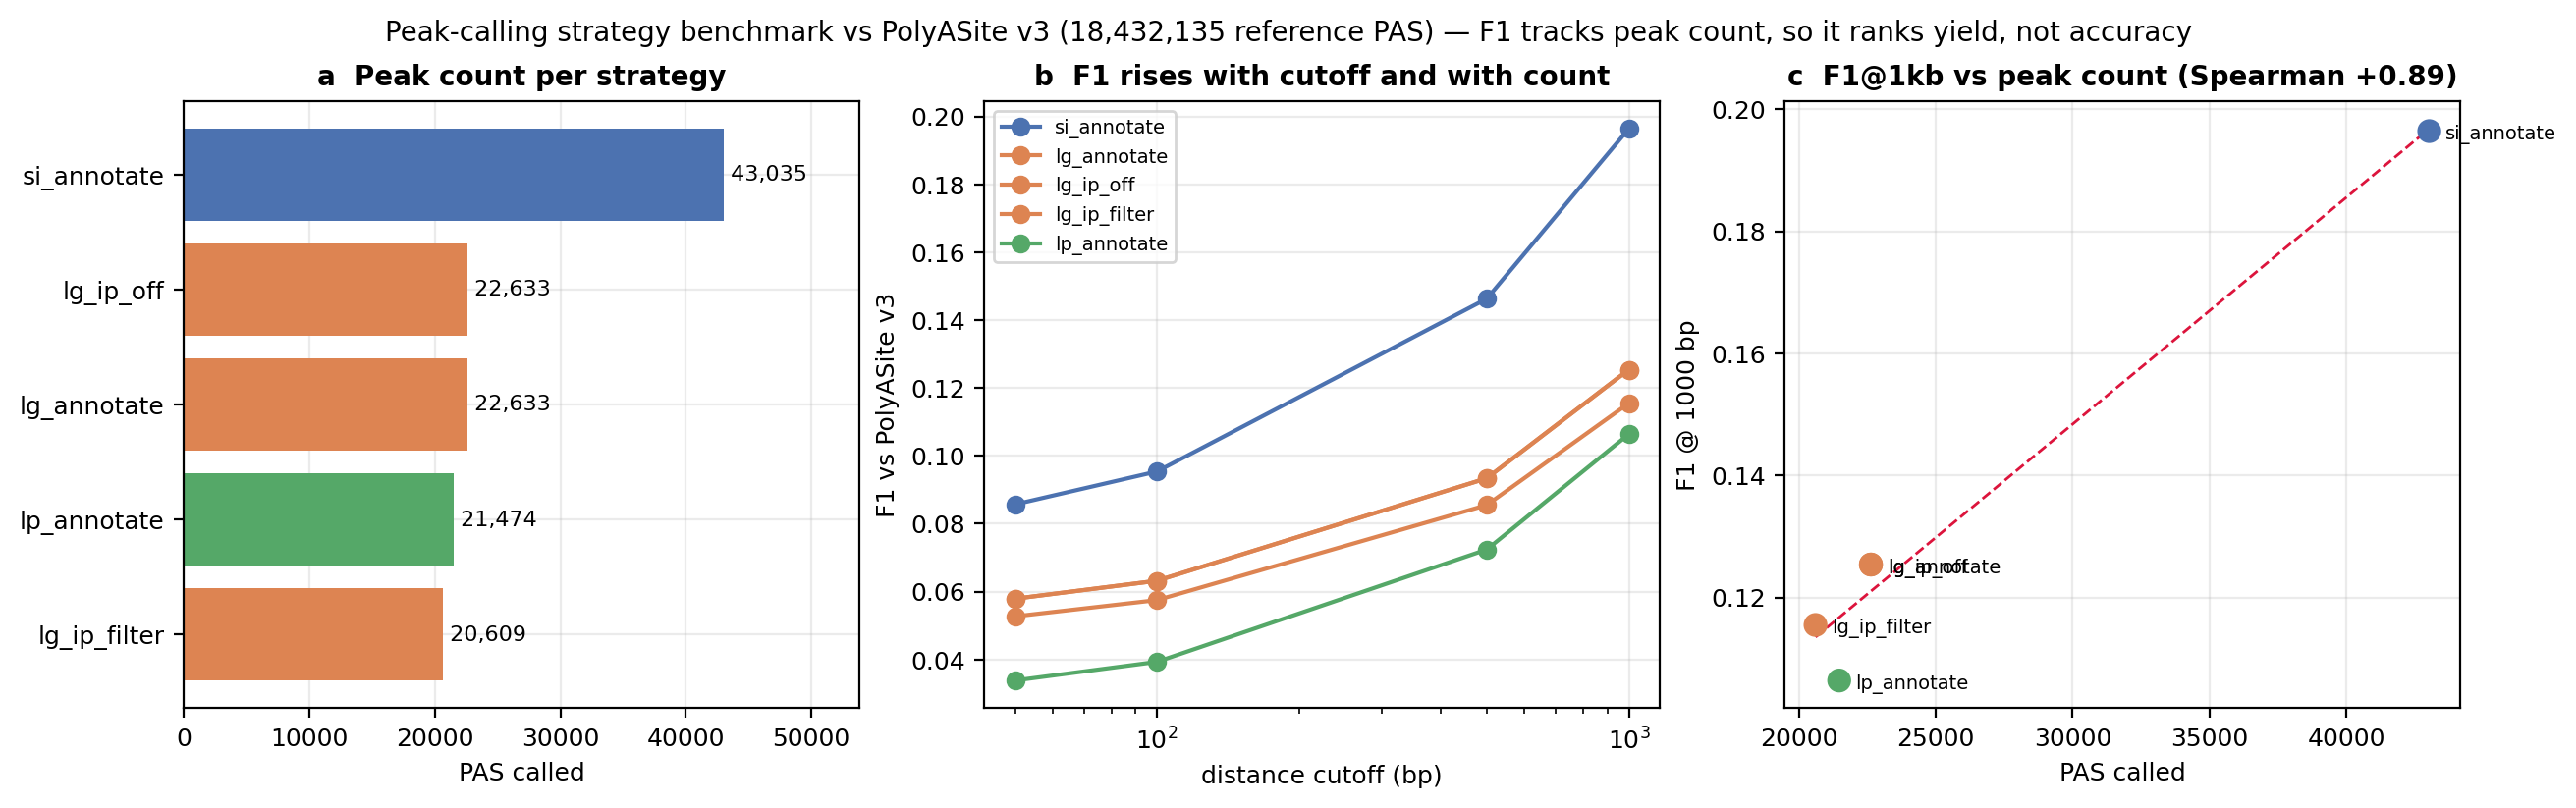
\includegraphics[width=\textwidth]{figures/corrected/01_strategy_benchmark.png}
  \caption{Peak count (a), F1 across cutoffs (b), and F1@1kb against peak count
    (c). Panel (c) is the result that matters: across the five configurations F1
    and peak count are rank-identical.}
  \label{fig:strategy_benchmark}
\end{figure}

\subsection{Why This Ranking Does Not Measure Accuracy}

Precision against PolyASite v3 is \textbf{0.9964 at 50\,bp and 0.9994 at
1000\,bp} --- for every strategy. With 18.4M reference entries the atlas tiles
the transcribed genome densely enough that essentially any call near a gene falls
within 50\,bp of \emph{some} annotated PAS. Precision is saturated and carries no
discriminative information.

\begin{figure}[htbp]
  \centering
  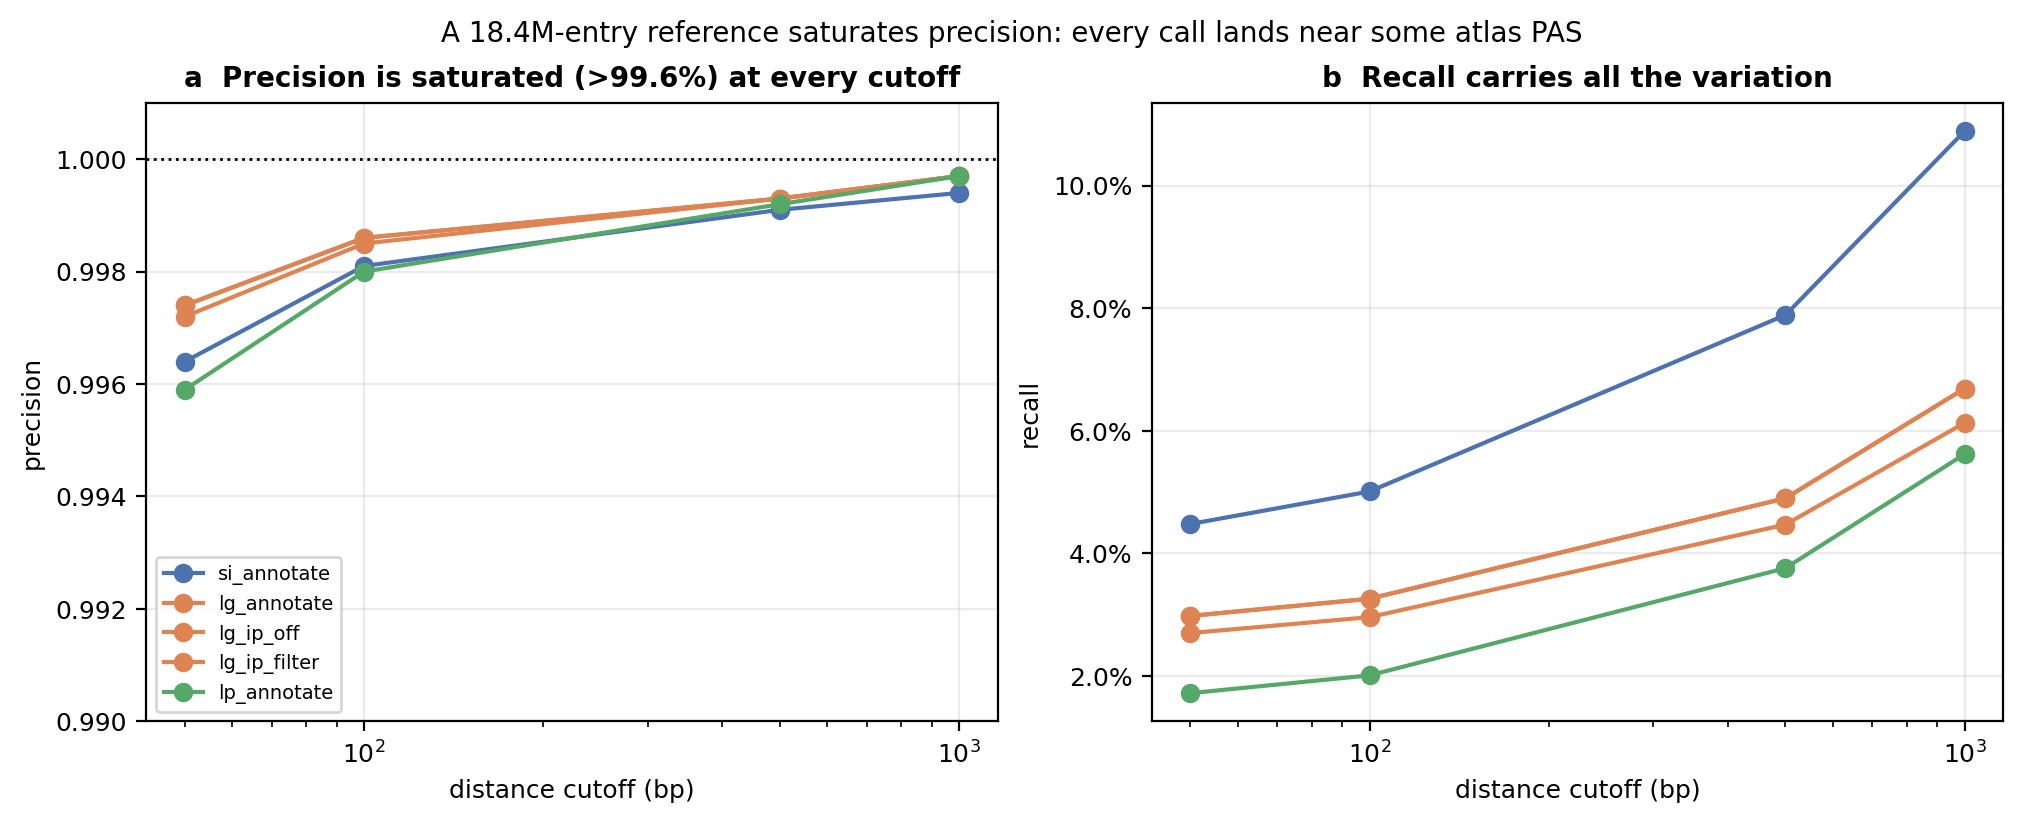
\includegraphics[width=\textwidth]{figures/corrected/02_atlas_saturation.png}
  \caption{Precision is pinned above 99.6\% at every cutoff (a) while recall
    supplies all the variation (b).}
  \label{fig:atlas_saturation}
\end{figure}

Because precision is constant, F1 reduces to a monotone function of recall, and
recall is the fraction of 18.4M reference PAS recovered --- which can only grow as
a strategy emits more peaks. Sierra-iterative ranks first because it calls
1.90$\times$ more PAS than lambda\_gradient, and gains 1.57$\times$ the F1.
\textbf{The ranking is a yield ranking, not an accuracy ranking.} This is the same
failure mode previously documented for peak width, reached through a different
statistic.

The corollary is that \texttt{lg\_ip\_filter} appears ``worse'' (F1 0.116 vs
0.125) purely because the internal-priming filter removes 2,024 peaks. A filter
that removes false positives is penalised by this metric. F1 against a saturated
reference must not be used to accept or reject a filtering step.

\subsection{Count-Controlled Comparison}

To separate caller quality from caller yield, every strategy is randomly
subsampled to the smallest strategy's peak count ($n = 20{,}609$; 20 replicates)
and positional agreement with the atlas recomputed, alongside the full distance
distribution from each called PAS to its nearest atlas entry.

\begin{figure}[htbp]
  \centering
  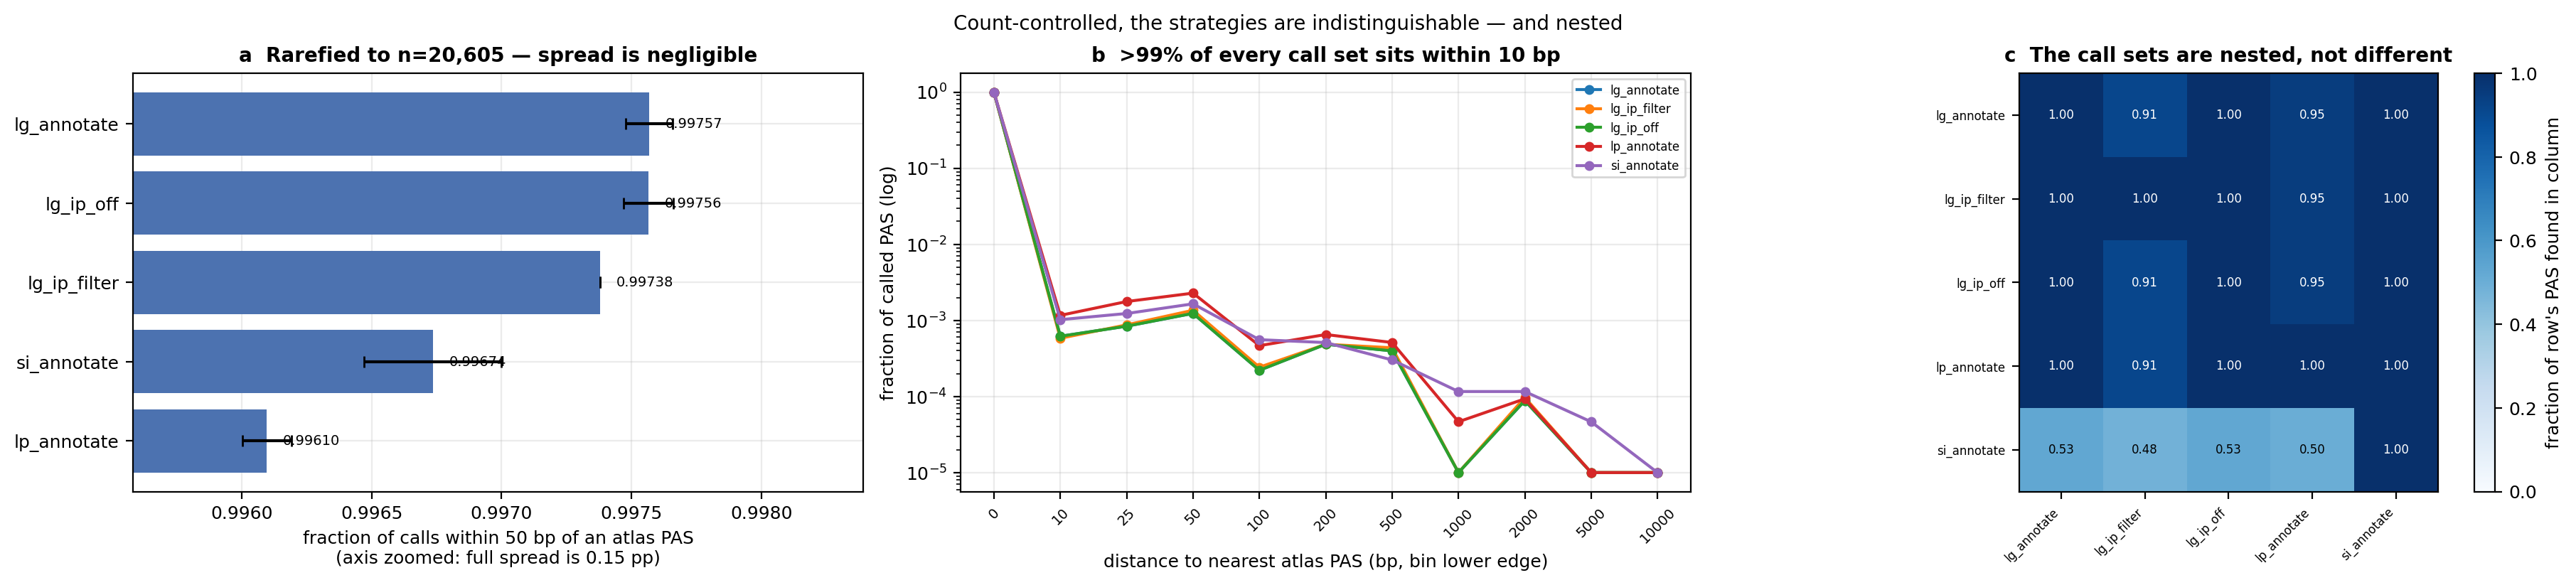
\includegraphics[width=\textwidth]{figures/corrected/03_count_controlled.png}
  \caption{(a) fraction of calls within 50\,bp of an atlas PAS after rarefying all
    strategies to $n = 20{,}605$ (200 replicates); (b) distance-to-nearest-atlas
    distribution; (c) pairwise containment between call sets.}
  \label{fig:count_controlled}
\end{figure}

\begin{table}[htbp]
  \centering
  \small
  \begin{tabular}{lrrr}
    \toprule
    run & frac.\ within 50\,bp (rarefied) & sd & median distance \\
    \midrule
    \texttt{lg\_annotate}   & 0.99757 & 0.00009 & 0\,bp \\
    \texttt{lg\_ip\_off}    & 0.99756 & 0.00010 & 0\,bp \\
    \texttt{lg\_ip\_filter} & 0.99738 & 0.00000 & 0\,bp \\
    \texttt{si\_annotate}   & 0.99674 & 0.00026 & 0\,bp \\
    \texttt{lp\_annotate}   & 0.99610 & 0.00009 & 0\,bp \\
    \bottomrule
  \end{tabular}
  \caption{Count-controlled positional agreement with PolyASite v3.}
  \label{tab:rarefaction}
\end{table}

\textbf{The count-controlled ranking inverts the F1 ranking.} With peak count held
fixed, lambda\_gradient (0.99757) edges out sierra\_iterative (0.99674) --- the
reverse of the F1 order. That confirms the F1 result was yield, not quality. But
the honest reading is stronger: \textbf{the entire spread is 0.15 percentage
points}, and the median distance to the nearest atlas PAS is \textbf{0\,bp for
every strategy}, with $>$99.3\% of all calls landing within 10\,bp.

\begin{quote}
\textbf{This benchmark cannot rank these callers --- by any of its statistics.}
Precision saturates, F1 measures yield, and count-controlled positional agreement
is identical to within 0.15\,pp. Choosing a peak caller requires an orthogonal
criterion: reproducibility across datasets, agreement with matched
3\textquotesingle{}-end sequencing, or downstream clustering stability --- none of
which is a distance-to-atlas statistic.
\end{quote}

\textbf{The call sets are nested, not different.} 100\% of lambda\_gradient's
22,633 PAS are found within 100\,bp in sierra's set, while only 53\% of sierra's
43,035 are found in lambda\_gradient's --- sierra is close to a strict superset.
Likewise \texttt{lg\_ip\_filter} $\subset$ \texttt{lg\_annotate} (100\% contained;
the filter only removes), and \texttt{lg\_annotate} $\equiv$ \texttt{lg\_ip\_off}
exactly (Jaccard 1.000). This supersedes the earlier claim that ``statistical
strategies find fundamentally different peaks'' --- on the corrected data they find
the same peaks, in differing amounts.

\subsection{Internal Priming and Annotation-Window Sensitivity}

\begin{figure}[htbp]
  \centering
  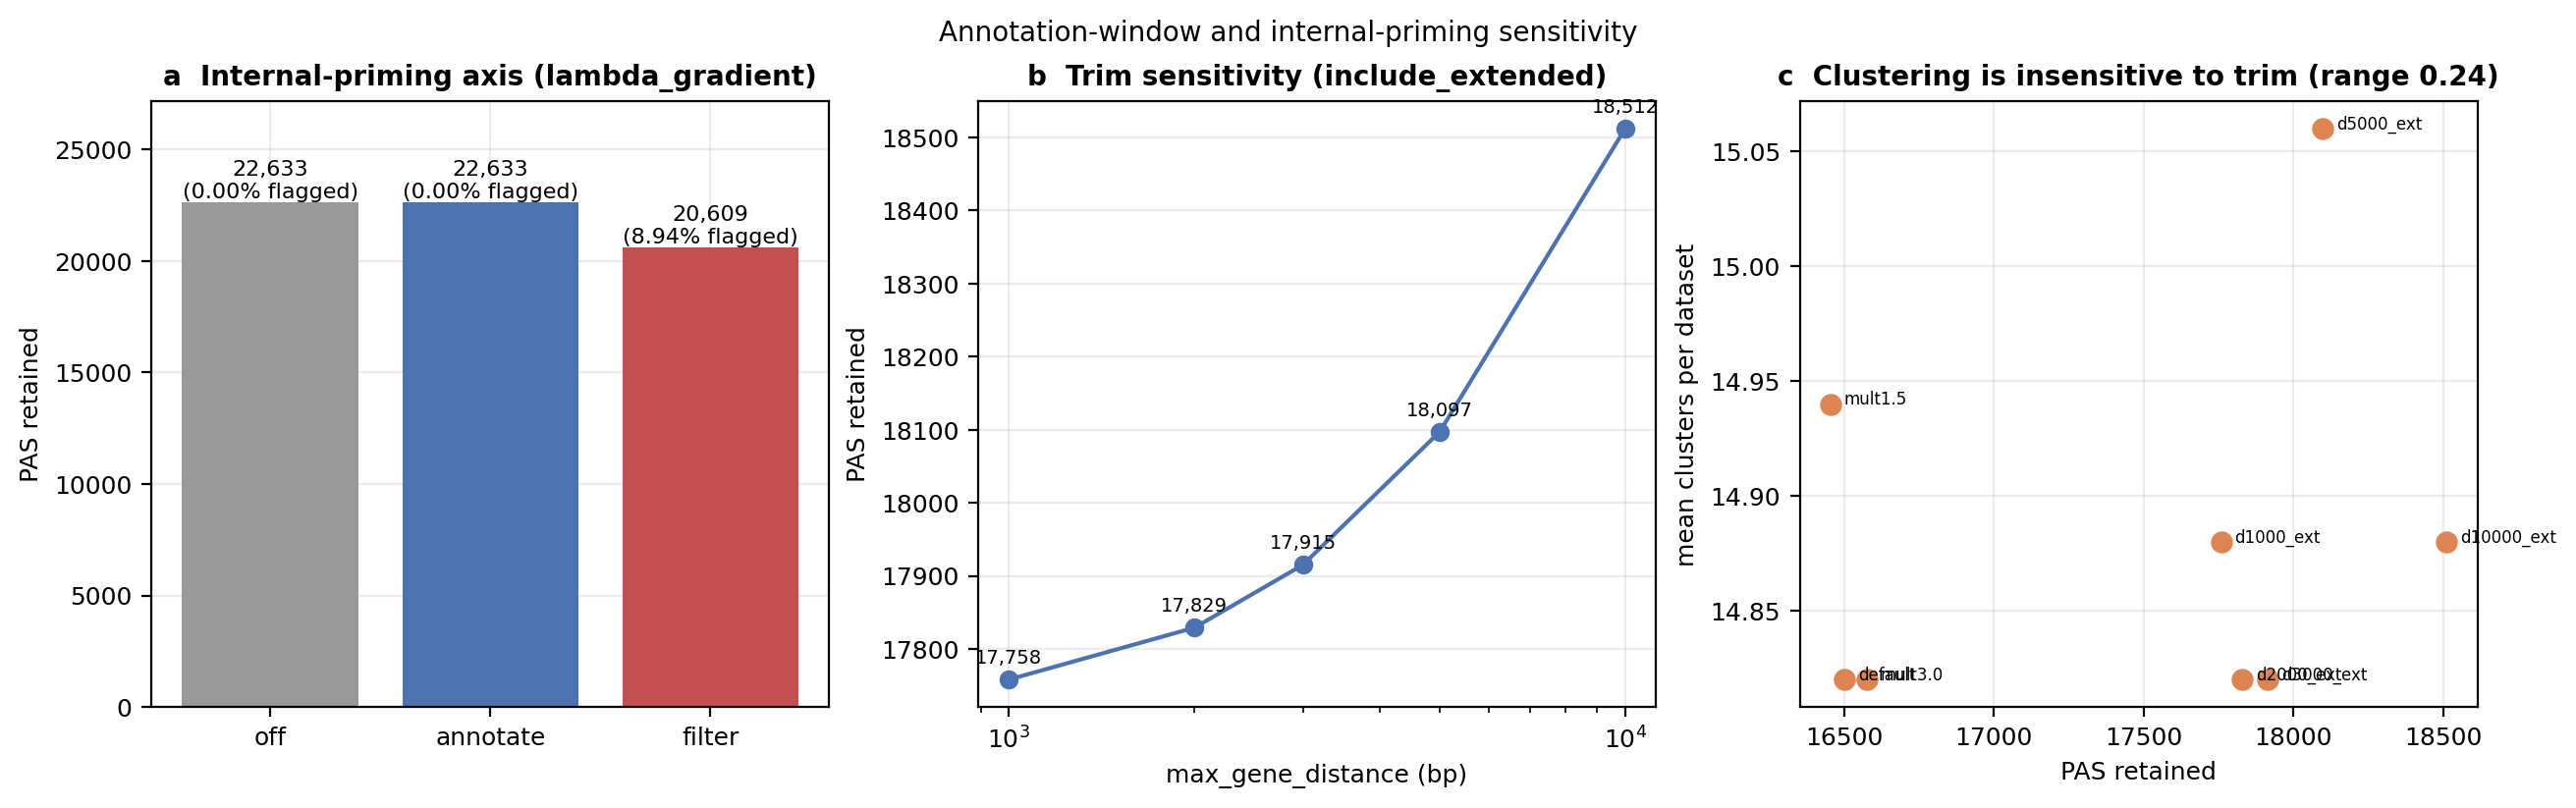
\includegraphics[width=\textwidth]{figures/corrected/04_ip_and_trim.png}
  \caption{(a) the internal-priming axis on lambda\_gradient --- the FASTA filter
    flags and removes 8.94\% of peaks (22,633 $\rightarrow$ 20,609);
    \texttt{annotate} and \texttt{off} are identical in peak count, so
    \texttt{filter} is the only mode that changes output. (b) widening
    \texttt{max\_gene\_distance} from 1\,kb to 10\,kb with
    \texttt{include\_extended} adds only 754 PAS. (c) mean clusters per dataset
    moves across a range of 0.24 over the whole trim grid.}
  \label{fig:ip_and_trim}
\end{figure}

% ─────────────────────────────────────────────────────────────────────────────
\section{Clustering (Under Development)}
\label{sec:clustering}
% ─────────────────────────────────────────────────────────────────────────────

\subsection{Method: TF-IDF + LSI + Leiden}

Peak data is sparse and binary-ish (like scATAC-seq), so we use the scATAC-seq
approach instead of standard gene expression normalisation.

\begin{figure}[htbp]
  \centering
  \includegraphics[width=0.85\textwidth]{figures/fig_tfidf_pipeline.png}
  \caption{TF-IDF + LSI clustering pipeline for PAS data.}
  \label{fig:tfidf_pipeline}
\end{figure}

\textbf{TF-IDF} (Signac Method 1):
\begin{itemize}
  \item TF = count / total\_counts\_per\_cell
  \item IDF = n\_cells / cells\_with\_peak
  \item Result = $\log_{1+x}(\mathrm{TF} \times \mathrm{IDF} \times 10{,}000)$
\end{itemize}

\textbf{LSI}: TruncatedSVD on sparse TF-IDF matrix. First component removed
(depth-correlated).

\textbf{Cosine distance} for k-NN: appropriate for sparse high-dimensional data.

\textbf{Leiden}: Replaces deprecated Louvain. Guarantees connected communities.

\subsection{Parameter Sensitivity and Agreement with Expression Labels}

\begin{figure}[htbp]
  \centering
  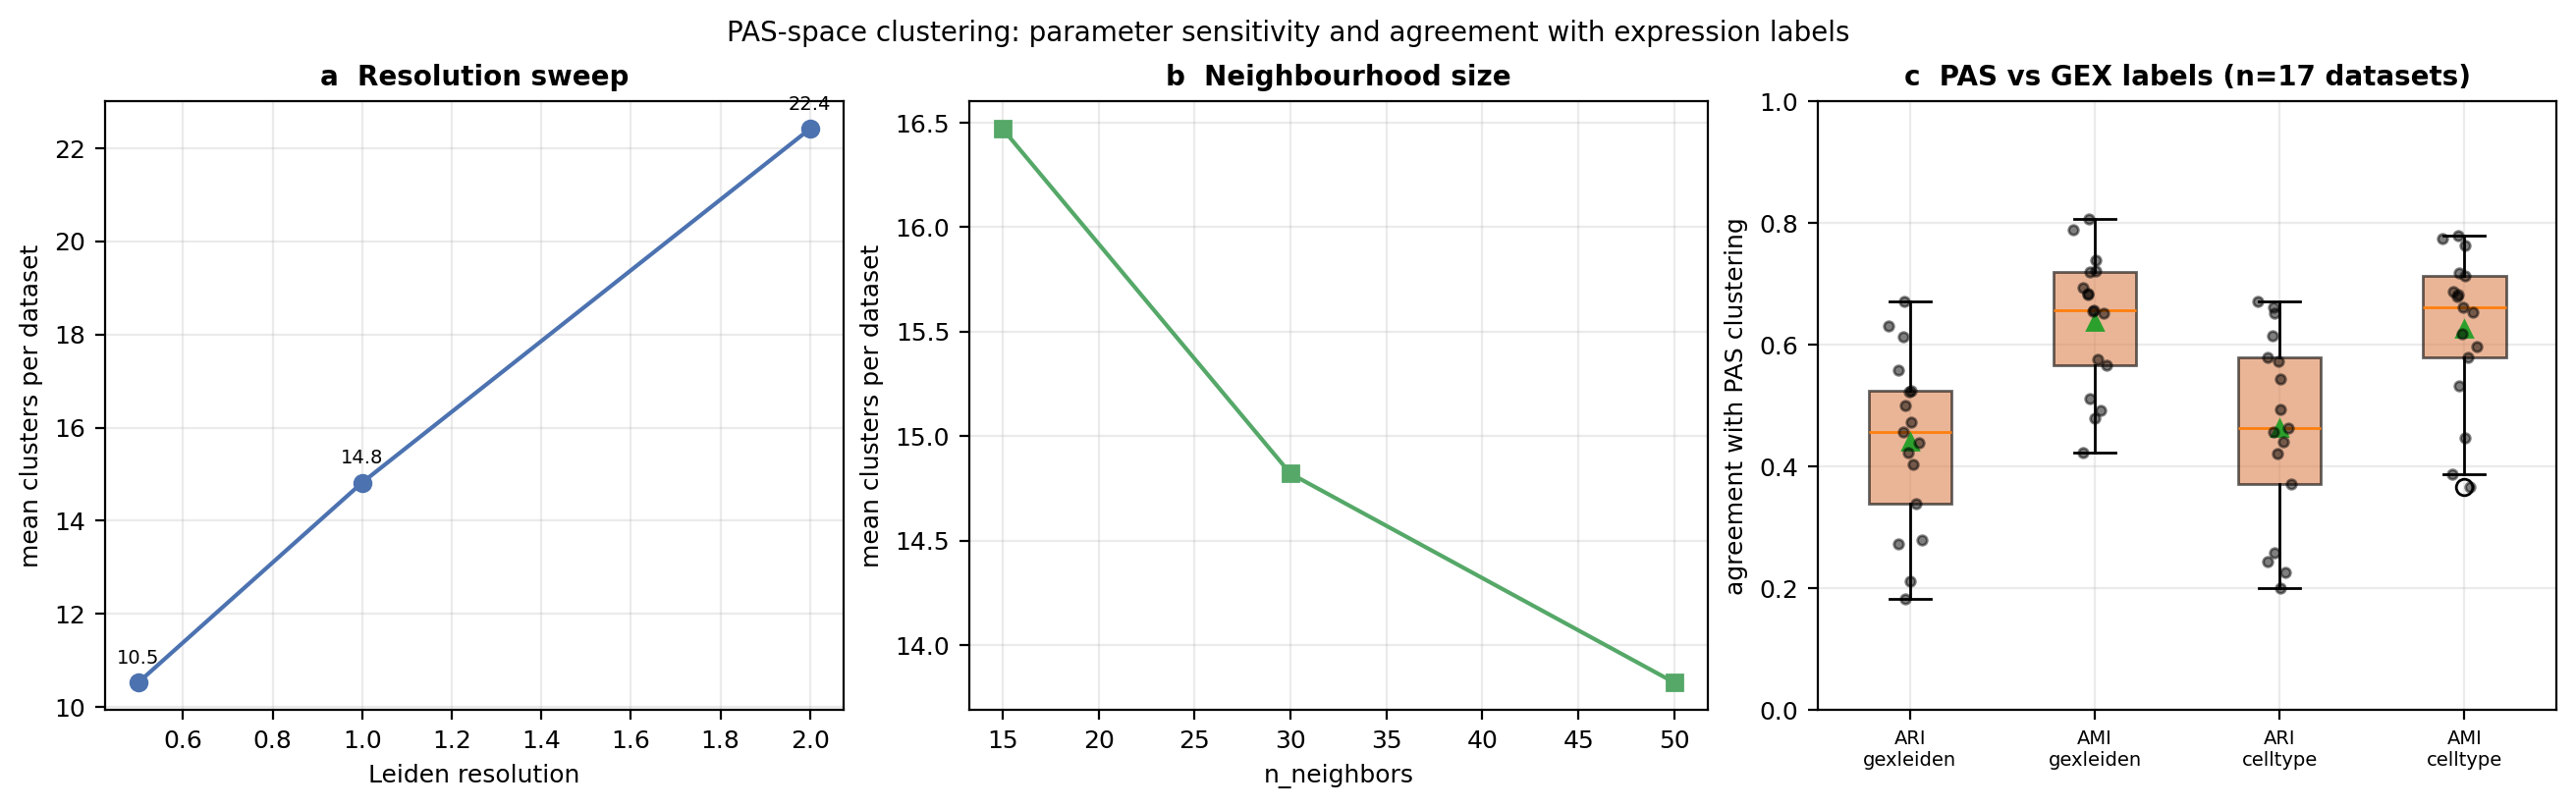
\includegraphics[width=\textwidth]{figures/corrected/05_clustering.png}
  \caption{(a) Leiden resolution against mean clusters per dataset across the
    17-dataset cohort: 0.5 $\rightarrow$ 10.53, 1.0 $\rightarrow$ 14.82,
    2.0 $\rightarrow$ 22.41. (b) neighbourhood size: \texttt{n\_neighbors}
    15 $\rightarrow$ 16.47, 30 $\rightarrow$ 14.82, 50 $\rightarrow$ 13.82.
    (c) agreement between PAS-space Leiden clustering and expression-side labels,
    one point per dataset.}
  \label{fig:clustering_corrected}
\end{figure}

\begin{table}[htbp]
  \centering
  \small
  \begin{tabular}{lrrr}
    \toprule
    comparison & mean & median & sd \\
    \midrule
    ARI, GEX-Leiden vs PAS      & 0.441 & 0.456 & 0.145 \\
    AMI, GEX-Leiden vs PAS      & 0.638 & 0.657 & 0.112 \\
    ARI, cell-type label vs PAS & \textbf{0.463} & 0.463 & 0.158 \\
    AMI, cell-type label vs PAS & \textbf{0.626} & 0.662 & 0.128 \\
    \bottomrule
  \end{tabular}
  \caption{Cohort concordance between PAS clustering and gene-expression
    clustering, $n = 17$ datasets.}
  \label{tab:gex_concordance}
\end{table}

\textbf{This supersedes the previously reported ARI $= 0.869$.} That figure came
from a single small test run whose cell count was inflated by the
barcode-collision bug; it is withdrawn. The corrected cohort value,
ARI $\approx 0.46$ / AMI $\approx 0.63$ across 17 independent datasets, is the
defensible number.

PAS-space clustering recovers substantial but \textbf{partial} structure relative
to expression. AMI (0.63) materially exceeds ARI (0.46), the signature of a
partition that is largely concordant but more finely split than the reference ---
consistent with, though not proof of, cells sharing an expression identity while
differing in polyadenylation. Establishing that claim requires showing the extra
splits are reproducible across datasets, which this sweep does not test.

Note also that \texttt{leiden\_libsize} yields more clusters than
\texttt{leiden\_tfidf} (16.82 vs 14.82 at matched resolution). Cluster count alone
does not rank the two normalisations; the earlier claim that ``TF-IDF beats
library-size at every resolution'' rested on the withdrawn single-run ARI and is
not re-established here.

% ─────────────────────────────────────────────────────────────────────────────
\section{Differential APA --- Switch Test}
\label{sec:switch_test}
% ─────────────────────────────────────────────────────────────────────────────

\begin{figure}[htbp]
  \centering
  \includegraphics[width=\textwidth]{figures/switch_strategy_explainer.png}
  \caption{Differential APA strategy overview cartoon. \textbf{(A)} Fisher within-gene:
    a $2{\times}2$ read-count table is tested per PAS, using the gene's other PAS as
    the background so the test is conditional on gene-level read allocation.
    \textbf{(B)} NB pairwise GLM: a Negative Binomial regression fits cluster as a
    covariate with library size as an offset; the $\beta_{\text{cluster}}$ coefficient
    captures the log-fold change with overdispersion modelled explicitly.
    \textbf{(C)} NB multi omnibus LRT: full model (all K clusters) vs.\ null model
    (intercept only); the likelihood ratio statistic follows $\chi^2(K{-}1)$ and
    gives one global variability p-value per PAS.}
  \label{fig:switch_explainer}
\end{figure}

\subsection{Why ``Differential APA'' is Statistically Tricky}

The naive approach --- applying a Fisher exact test to pseudo-bulk read totals per
PAS across all clusters --- has a fundamental pseudo-replication problem. A gene with
20 PAS produces 20 correlated tests, and any global read imbalance between clusters
inflates every individual p-value. On the v9 dataset the uncorrected Fisher flagged
9,197 significant PAS (out of 17,093 tested) for cluster 0 vs 1 --- a 54\% rate that
is biologically implausible. The within-gene framing corrects this: the $2{\times}2$
table for each PAS uses the gene's other PAS as the background, so the test asks
``conditional on reads allocated to this gene, does this PAS get used
disproportionately?'' rather than ``does this PAS carry more total reads?''. The
within-gene Fisher is the design used by DEXSeq for splicing and is now the default in
PeakATail's \texttt{fisher} strategy.

\subsection{Fisher (Within-Gene)}

For each gene $G$ and each PAS $p \in G$, the test is on the $2{\times}2$ read-count
table:

\begin{lstlisting}
                  cluster1      cluster2
reads at PAS p    r_p,c1        r_p,c2
reads at other    R_G,c1-r_p    R_G,c2-r_p
\end{lstlisting}

where $R_{G,ci}$ is the total reads at all PAS of gene $G$ in cluster $ci$. Genes
with fewer than 2 PAS are excluded. BH FDR is applied across all tested PAS after
collecting results from all genes.

Effect size columns:
\begin{itemize}
  \item \texttt{delta\_proportion} $= (r_{p,c1}/R_{G,c1}) - (r_{p,c2}/R_{G,c2})$:
        signed change in within-gene proportion.
  \item \texttt{log2fc}: $\log_2$ of the proportion ratio (with an $\varepsilon$ floor
        to avoid $\log(0)$).
  \item \texttt{odds\_ratio}: from \texttt{scipy.stats.fisher\_exact}.
\end{itemize}

\textbf{When to use}: Fast (no GLM fit), exact (no asymptotic approximation), works
with any cluster size. Best first-pass scan for 2-cluster comparisons when the primary
goal is ranking genes rather than quantifying effect sizes. The within-gene framing is
statistically correct but the p-values are still anti-conservative for overdispersed
scRNA-seq counts because Fisher assumes fixed marginals.

\textbf{Implementation}: \texttt{ema/switch\_test/strategies/fisher.py :: FisherStrategy}.

\subsection{NB Pairwise}

For each PAS independently, a Negative Binomial GLM is fitted:

\[
  \log(\mu_{ij}) = \beta_0 + \beta_{\text{cluster}} \cdot \mathbf{1}[\text{cell } j \in \text{cluster}_2] + \log(\text{library\_size}_j)
\]

where $\mu_{ij}$ is the expected count for PAS $i$ in cell $j$, $\mathbf{1}(\cdot)$
is the cluster indicator, and $\log(\textit{library\_size}_j)$ is an offset (not a free
parameter --- it normalises for sequencing depth per cell). The NB dispersion
parameter $\alpha$ is estimated per PAS via maximum likelihood
(\texttt{NegativeBinomial.fit} from~statsmodels), falling back to method-of-moments if
the MLE fails to converge:

\[
  \hat{\alpha}_{\mathrm{MOM}} = \frac{s^2 - \bar{x}}{\bar{x}^2}
\]

The Wald z-test on the $\beta_{\text{cluster}}$ coefficient gives the p-value. BH FDR
is applied across all tested PAS.

\textbf{Why NB over Poisson}: In scRNA-seq, variance $\gg$ mean (overdispersion).
Poisson assumes variance = mean; NB adds the quadratic term $\alpha \mu^2$ so
$\mathrm{Var} = \mu + \alpha \mu^2$. Using Poisson inflates test statistics and
produces anti-conservative p-values. NB is the standard model in DESeq2, edgeR, and
all modern bulk RNA-seq pipelines and extends cleanly to single-cell pseudo-bulk.

\textbf{When to use}: When sample sizes are large enough for NB MLE to converge
reliably ($\geq 30$ cells per cluster recommended), and when quantified effect sizes
with confidence intervals are needed (the \texttt{log2fc} column maps directly to
$\beta_{\text{cluster}} / \log 2$). Slower than Fisher (GLM fit per PAS), but more
principled.

\textbf{Implementation}: \texttt{ema/switch\_test/strategies/nb\_pairwise.py}\\
\hspace*{1em}\texttt{:: NbPairwiseStrategy}. Uses \texttt{joblib.Parallel(backend="loky")} over PAS batches.

\subsection{NB Multi (Omnibus)}

The omnibus test fits two GLMs per PAS across all $K$ clusters:

\begin{itemize}
  \item \textbf{Full model}: \texttt{count $\sim$ C(cluster) + offset(log(library\_size))}
        --- one coefficient per cluster ($K{-}1$ indicator columns + intercept).
  \item \textbf{Null model}: \texttt{count $\sim$ 1 + offset(log(library\_size))}
        --- intercept only.
\end{itemize}

The likelihood ratio test (LRT) statistic:

\[
  \mathrm{LRT} = 2 \cdot (LL_{\text{full}} - LL_{\text{null}}) \;\sim\; \chi^2(K{-}1)
\]

gives an omnibus p-value: a significant PAS is one where \emph{any} cluster shows
differential usage, regardless of direction or which cluster pair drives it. This is
analogous to a one-way ANOVA generalised to NB counts. No \texttt{log2fc} column is
emitted; if directionality matters, the full-model cluster coefficients must be
inspected separately.

\textbf{When to use}: Multi-cluster screening where you want a single global
variability statistic per PAS --- e.g., to build a ranked list of PAS to follow up,
or to filter the count matrix before downstream analysis. NB multi is the most
computationally expensive strategy (two GLM fits per PAS, each with $K{-}1$
coefficients) but produces one interpretable statistic that does not require choosing
cluster pairs.

\textbf{Note}: The \texttt{nb\_multi} q-values on this v9 dataset are extremely small
(median $9 \times 10^{-10}$) because the test uses all 12 clusters simultaneously ---
even tiny inter-cluster variation becomes highly significant with 1,051 cells. This is
expected behaviour, not a bug.

\textbf{Implementation}: \texttt{ema/switch\_test/strategies/nb\_multi.py :: NbMultiStrategy}.

\subsection{Strategy Comparison on the v9 Run}

Comparison on cluster 0 vs 1 (pair chosen because it has the largest cell counts:
213 cells in C0, 183 in C1):

\begin{figure}[htbp]
  \centering
  \includegraphics[width=\textwidth]{figures/switch_strategy_real_data.png}
  \caption{\textbf{[PRE-FIX RUN --- illustrative only.]} This figure shows output \emph{format} from the superseded v9 run; its values predate the cell-doubling and atlas-snap fixes and must not be cited. (A) Significant PAS at $q{<}0.05$ per strategy. Fisher flags $\sim$9,200
    PAS --- 10$\times$ more than NB pairwise (451), reflecting its anti-conservative
    character. NB multi's 19,832 reflects the omnibus nature (tested against all 12
    clusters). (B) Jaccard similarity between Fisher and NB-pairwise significant sets
    = 0.027 --- very low concordance, confirming that Fisher is capturing many false
    positives absent in the NB GLM. (C) Score distribution: NB pairwise q-values are
    concentrated near 1.0 (most PAS not significant), while Fisher spreads across the
    entire range.}
  \label{fig:switch_strategy_real_data}
\end{figure}

\begin{table}[htbp]
  \centering
  \caption{Strategy comparison on v9 run, cluster 0 vs 1.}
  \label{tab:switch_strategy_comparison}
  \resizebox{\textwidth}{!}{%
  \begin{tabular}{lrrrrr}
    \toprule
    \textbf{Strategy} & \textbf{n\_tested} & \textbf{n\_sig ($q{<}0.05$)} &
    \textbf{n\_sig\_strong} & \textbf{Jaccard vs NB-pair} & \textbf{Runtime (s)} \\
    \midrule
    fisher      & 17,093 & 9,197  & 8,176  & 0.027 & 7   \\
    nb\_pairwise & 1,289  & 451    & 402    & 1.0   & 3   \\
    nb\_multi    & 20,274 & 19,832 & 19,832 (omnibus) & ---   & 227 \\
    \bottomrule
  \end{tabular}}
\end{table}

\noindent\textit{NB pairwise tests only 1,289 PAS because the
\texttt{min\_cells\_per\_group=10} filter on non-zero cells is applied per PAS per
cluster (cell-level non-zero counts, not total cell count). Fisher tests 17,093
because it uses aggregated counts and only requires $\geq 10$ total cells per cluster.}

\subsection{When to Use Which}

\begin{table}[htbp]
  \centering
  \caption{Differential APA strategy selection guide.}
  \label{tab:switch_guide}
  \begin{tabularx}{\textwidth}{lX}
    \toprule
    \textbf{Need} & \textbf{Use} \\
    \midrule
    Fast first-pass scan, 2 clusters, exact test &
      \texttt{fisher} \\
    Effect sizes with CIs, NB-correct p-values, large clusters ($\geq$30 cells) &
      \texttt{nb\_pairwise} \\
    Single global variability stat per PAS, multi-cluster screening &
      \texttt{nb\_multi} \\
    Ranking genes (not PAS) for follow-up &
      Any --- aggregate by gene after FDR \\
    \bottomrule
  \end{tabularx}
\end{table}

% ─────────────────────────────────────────────────────────────────────────────
\section{3\textquotesingle UTR Length Quantification}
\label{sec:length}
% ─────────────────────────────────────────────────────────────────────────────

\begin{figure}[htbp]
  \centering
  \includegraphics[width=\textwidth]{figures/length_strategy_explainer.png}
  \caption{3$'$UTR length quantification strategy overview cartoon.
    \textbf{(A)} Classic PDUI: uses only the proximal (P) and distal (D) PAS;
    PDUI = D/(P+D), ranging from 0 (short 3$'$UTR) to 1 (long 3$'$UTR).
    \textbf{(B)} Proportion per-gene: stacked bar showing per-PAS usage fractions
    across all detected PAS for a gene; captures the full distribution shift, not
    just a proximal/distal contrast.
    \textbf{(C)} Proportion per-isoform: proportions computed within each
    transcript isoform's PAS set, allowing isoform-specific budgeting of reads.
    \textbf{(D)} Shannon entropy: $H = -\sum_i p_i \log_2 p_i$ summarises
    concentration of PAS usage; low entropy = one dominant site, high entropy =
    diversified usage across PAS.}
  \label{fig:length_explainer}
\end{figure}

\subsection{Why Quantify 3\textquotesingle UTR Length?}

Alternative polyadenylation changes the length of the 3\textquotesingle UTR, altering
the density of regulatory elements in that region. Shorter 3\textquotesingle UTRs lose
miRNA binding sites (often hundreds of predicted targets per transcript), AU-rich
elements that govern mRNA stability, and RNA-binding protein motifs. This allows the
transcript to escape post-transcriptional repression --- a mechanism observed in tumour
cells (Mayr \& Bartel 2009), activated immune cells (Sandberg et al.\ 2008), and
during neuronal differentiation (Agarwal et al.\ 2021). Quantifying 3\textquotesingle
UTR length per cell cluster therefore reports on a layer of gene regulation that is
invisible to standard gene expression analysis.

\subsection{Classic PDUI}

\textbf{Proximal-Distal Usage Index} was introduced by scAPA and is the default metric
in DaPars2. For a gene with a proximal PAS (P) and a distal PAS (D):

\[
  \mathrm{PDUI} = \frac{\text{distal\_reads}}{\text{proximal\_reads} + \text{distal\_reads}}
\]

PDUI = 0 means all reads at the proximal site (short 3\textquotesingle UTR); PDUI = 1
means all reads at the distal site (long 3\textquotesingle UTR). For genes with more
than 2 PAS, PeakATail selects the first PAS as proximal and the last as distal in
transcription order (strand-aware). Genes with only one detected PAS are excluded.

\textbf{Limitation}: The 2-PAS reduction discards information from all intermediate
PAS. For a gene with 5 PAS, PDUI only uses 2, ignoring 3 sites that may be
biologically meaningful. On the v9 data (lambda\_gradient strategy), classic PDUI
quantified 1,898 genes (out of 5,407 with $\geq$1 PAS in \texttt{adata.var}),
mean PDUI $0.50 \pm 0.48$.

\textbf{When to use}: Historical comparison with DaPars/scAPA results, or when a
single scalar per gene is sufficient and the gene set of interest is mostly 2-PAS.

\begin{figure}[htbp]
  \centering
  \includegraphics[width=0.85\textwidth]{figures/length_pdui_distribution_classic.png}
  \caption{\textbf{[PRE-FIX RUN --- illustrative only.]} Values predate the cell-doubling and atlas-snap fixes and must not be cited; see figure~fig:length_strategy for the corrected-sweep equivalent. Classic PDUI distribution across all quantified genes on the v9 dataset, produced by \texttt{ema switch length --strategy classic}. The bimodal shape (peaks near 0 and 1) reflects the proximal-dominant vs distal-dominant gene populations expected of pseudo-bulk APA.}
  \label{fig:length_pdui_dist}
\end{figure}

\begin{figure}[htbp]
  \centering
  \includegraphics[width=\textwidth]{figures/length_shifts_classic_cluster_pairs.png}
  \caption{\textbf{[PRE-FIX RUN --- illustrative only.]} Values predate the cell-doubling and atlas-snap fixes and must not be cited; see figure~fig:length_strategy for the corrected-sweep equivalent. Per-gene PDUI shift across every cluster pair (rows = genes, columns = cluster pairs). Red indicates \emph{lengthening} (higher PDUI in the first cluster of the pair); blue indicates \emph{shortening}. This is the canonical visualisation of 3\textquotesingle UTR shorten/lengthen signal across the clustered cell population. Output of the \texttt{length\_shifts} viz strategy that fires automatically after \texttt{ema switch length --strategy classic}.}
  \label{fig:length_shifts}
\end{figure}

\subsection{Proportion per Gene}

A generalisation that uses all detected PAS. For each gene $G$ and each cell $j$, the
proportion at PAS $i$ is:

\[
  p_{i,j} = \frac{\text{reads}_{i,j}}{\sum_k \text{reads}_{k,j}}
  \quad (\text{sum over all PAS } k \text{ of gene } G)
\]

This produces a vector of proportions summing to 1.0 per (gene, cell). In the
long-format output, each row is one (gene, PAS, cell) triplet. The vector captures the
full distribution of usage, not just the proximal/distal contrast.

\textbf{When to use}: When genes have 3+ PAS and you want to capture the entire
distribution shift (not just a scalar summary). The output is high-dimensional --- one
vector per (gene, cell) --- so downstream analysis typically summarises with the
highest-proportion PAS per cluster or performs Jensen-Shannon divergence between
cluster distributions.

On the v9 data (lambda\_gradient strategy): 5,407 genes quantified, mean proportion
$0.30 \pm 0.44$. Zero genes hit the inter-cluster proportion shift threshold of $> 0.1$
under the strict mean-across-PAS metric --- proportion is vector-valued and the scalar
reduction rarely exceeds the threshold even when individual PAS proportions swing
substantially.

\begin{figure}[htbp]
  \centering
  \includegraphics[width=\textwidth]{figures/length_proportion_heatmap.png}
  \caption{\textbf{[PRE-FIX RUN --- illustrative only.]} Values predate the cell-doubling and atlas-snap fixes and must not be cited; see figure~fig:length_strategy for the corrected-sweep equivalent. Proportion-per-gene heatmap from \texttt{ema switch length --strategy proportion}. Each row is a (gene, PAS) entry; each column is a cluster; cell colour is the mean within-gene proportion of that PAS in that cluster. Genes with strong cluster-specific PAS choice appear as horizontal bands of contrasting colour.}
  \label{fig:length_proportion_heatmap}
\end{figure}

\subsection{Proportion per Isoform}

The same proportion formula as Section~\ref{sec:length}.3 (Proportion per Gene), but
the denominator sums only reads assigned to PAS belonging to a specific transcript
isoform. This requires the GTF to define which PAS fall within each isoform's
3\textquotesingle UTR, and a PAS-to-isoform mapping produced by
\texttt{ema.quantification.pas\_to\_isoform.map\_pas\_to\_isoforms}. The computation:

\[
  p_{i,j,t} = \frac{\text{reads}_{i,j}}{\sum_{k \in \text{isoform } t} \text{reads}_{k,j}}
\]

\textbf{When to use}: When the biology concerns specific isoform usage rather than the
gene-level average --- e.g., transcript switching in splicing-coupled APA where a
switch in splice site changes which PAS are accessible. Requires GTF annotation with
transcript-level 3\textquotesingle UTR features.

\textbf{Note}: Per-isoform quantification was not benchmarked on this dataset due to
memory constraints (the GTF parsing + per-isoform matrix computation exceeds the 15 GB
RAM available on the test machine). The infrastructure is implemented and tested on
synthetic data.

\subsection{Shannon Entropy}

For each (gene, cell), Shannon entropy over PAS proportions:

\[
  H = -\sum_i p_i \cdot \log_2(p_i) \quad (\text{bits})
  \qquad
  H_{\text{norm}} = \frac{H}{\log_2 N} \quad (N = \text{number of PAS with } p_i > 0)
\]

Boundary cases:
\begin{itemize}
  \item $H = 0$: all reads at one PAS (maximally concentrated usage).
  \item $H = \log_2 N$: uniform distribution across all $N$ PAS (maximal diversity).
  \item $H_{\text{norm}} \in [0, 1]$ regardless of how many PAS the gene has,
        enabling cross-gene comparison.
\end{itemize}

Shannon entropy is a scalar per (gene, cell) --- one number that summarises the spread
of PAS usage without requiring a direction (proximal vs distal). It detects when a
cluster has concentrated usage on one PAS (low $H$) vs diversified usage across many
PAS (high $H$), independent of which PAS dominates.

\textbf{When to use}: Screening for genes where PAS usage becomes more or less
concentrated across conditions, without committing to a proximal/distal framing. High
$H$ genes are candidates for regulatory complexity; low $H$ genes in one condition but
high $H$ in another indicate condition-specific PAS concentration.

On the v9 data (lambda\_gradient strategy): 5,407 genes quantified, mean entropy
$0.14 \pm 0.39$ bits. 1,372 genes showed inter-cluster entropy shift $> 0.1$ bits.

\begin{figure}[htbp]
  \centering
  \includegraphics[width=0.85\textwidth]{figures/length_entropy_distribution_shannon.png}
  \caption{\textbf{[PRE-FIX RUN --- illustrative only.]} Values predate the cell-doubling and atlas-snap fixes and must not be cited; see figure~fig:length_strategy for the corrected-sweep equivalent. Shannon entropy distribution across all (gene, cell) pairs on the v9 dataset, produced by \texttt{ema switch length --strategy shannon}. Heavy concentration near 0 bits indicates most cells use a single dominant PAS per gene; the right tail captures cells with diversified usage.}
  \label{fig:length_entropy_dist}
\end{figure}

\subsection{Strategy Comparison on the v9 Run}

\begin{figure}[htbp]
  \centering
  \includegraphics[width=\textwidth]{figures/length_strategy_real_data.png}
  \caption{\textbf{[PRE-FIX RUN --- illustrative only.]} This figure shows output \emph{format} from the superseded v9 run; its values predate the cell-doubling and atlas-snap fixes and must not be cited. (A) Mean score per strategy with standard deviation bars. Classic PDUI has
    the widest spread (bimodal: proximal-dominant and distal-dominant genes). Shannon
    entropy is concentrated near 0 (most cells have concentrated usage). (B) Number of
    quantifiable units per strategy --- classic excludes multi-PAS-only genes. (C)
    Units with inter-cluster shift $> 0.1$. Classic has the highest count (4,045)
    because its bimodal nature makes any shift cross the 0.1 threshold easily. Shannon:
    2,948 genes. (D) PDUI distribution across clusters showing the characteristic
    U-shape.}
  \label{fig:length_strategy_real_data}
\end{figure}

\begin{table}[htbp]
  \centering
  \caption{Length strategy comparison on v9 run.}
  \label{tab:length_strategy}
  \begin{tabular}{llrrrr}
    \toprule
    \textbf{Strategy} & \textbf{Agg} & \textbf{n\_units} & \textbf{mean\_score} &
    \textbf{score\_std} & \textbf{n\_shift ($>$0.1)} \\
    \midrule
    classic     & per\_gene     & 1,898 & 0.501 & 0.481 & 1,895 \\
    proportion  & per\_gene     & 5,407 & 0.297 & 0.436 & 0     \\
    shannon     & per\_gene     & 5,407 & 0.136 & 0.393 & 1,372 \\
    proportion  & per\_isoform  & ---   & ---   & ---   & not run (RAM) \\
    \bottomrule
  \end{tabular}
\end{table}

\subsection{When to Use Which}

\begin{table}[htbp]
  \centering
  \caption{Length quantification strategy selection guide.}
  \label{tab:length_guide}
  \begin{tabularx}{\textwidth}{lX}
    \toprule
    \textbf{Goal} & \textbf{Use} \\
    \midrule
    Compare to DaPars / scAPA literature & \texttt{classic} \\
    Full distribution of $N$ PAS per gene & \texttt{proportion per\_gene} \\
    Isoform-specific PAS budgets & \texttt{proportion per\_isoform} \\
    Detect concentration changes (any direction) & \texttt{shannon} \\
    Combine scalar + distribution & \texttt{classic} + \texttt{proportion per\_gene} \\
    \bottomrule
  \end{tabularx}
\end{table}

% ─────────────────────────────────────────────────────────────────────────────
\section{Cross-Dataset Cluster Matching}
\label{sec:cross_dataset_match}
% ─────────────────────────────────────────────────────────────────────────────

\subsection{Motivation}

A single-cell APA experiment rarely stops at one sample. Comparing polyadenylation
profiles across biological conditions (treatment vs.\ control), sequencing protocols
(10x v2 vs.\ v3), or time-points requires that the cluster labels assigned independently
in each dataset be \emph{harmonised} into a shared canonical ID space before
differential or trajectory analyses are applied. Without harmonisation, ``cluster 0''
in dataset A may correspond to ``cluster 5'' in dataset B --- two names for the same
cell population. PeakATail addresses this through a pluggable cross-dataset matching
registry in \texttt{ema/clustering/cross\_dataset/}.

Three strategies are registered:

\begin{itemize}
  \item \textbf{marker\_overlap}: Wilcoxon marker PAS $\rightarrow$ Jaccard similarity
        matrix $\rightarrow$ Hungarian assignment
  \item \textbf{jaccard}: direct Jaccard overlap of cell barcode sets (shared-cell scenarios)
  \item \textbf{mnn}: Mutual Nearest Neighbours in a joint LSI embedding
\end{itemize}

All three strategies share the same abstract interface (\texttt{ClusterMatchStrategy.match})
and return a standardised \texttt{DataFrame} with columns \texttt{dataset\_id},
\texttt{original\_cluster}, \texttt{canonical\_cluster} (integer, dense, starting at 1),
\texttt{match\_confidence} ($\in [0, 1]$), and \texttt{matched\_to} (JSON list of
cross-dataset partners). Single-dataset inputs receive an identity mapping (confidence = 1.0,
no partners). Transitive closure is applied so that matched pairs across three or more
datasets correctly propagate: if $A_i \sim B_j$ and $B_j \sim C_k$, all three share
one canonical ID.

\begin{figure}[htbp]
  \centering
  \includegraphics[width=\textwidth]{figures/match_strategy_explainer.png}
  \caption{Cross-dataset cluster matching strategies. \textbf{(A)} Marker overlap:
    each cluster's fingerprint is its top-$N$ marker PAS (by Wilcoxon score); Jaccard
    similarity between fingerprints drives the Hungarian assignment across dataset pairs.
    \textbf{(B)} Jaccard cell-set: a bipartite graph of cluster pairs with edge weights
    equal to barcode-set Jaccard similarity; thick edges indicate high cell overlap.
    Only applicable when the same cells appear in both datasets.
    \textbf{(C)} MNN in shared LSI space: cells from all datasets are embedded jointly
    by TruncatedSVD; mutual nearest-neighbour pairs (each cluster is in the other's
    $k$-NN list) determine cluster-level similarity, then Hungarian assignment is applied.}
  \label{fig:match_explainer}
\end{figure}

\subsection{Strategy 1: Marker Overlap}
\label{sec:match_marker_overlap}

\textbf{Implementation}: \texttt{ema/clustering/cross\_dataset/marker\_overlap.py}\\
\phantom{\textbf{Implementation}: }\texttt{MarkerOverlapStrategy}

\textbf{Algorithm}:
\begin{enumerate}
  \item For each dataset, compute per-cluster marker PAS via Wilcoxon
        rank-sum (\texttt{rank\-\_genes\-\_groups}). The top-$N$ PAS by
        score form the cluster ``fingerprint''. Raw matrices are
        log-normalised if data looks raw (integer or $\max > 20$).
  \item For every pair of datasets $(A, B)$, build the Jaccard matrix
        between cluster fingerprints:
        \[
          J(A_i, B_j) = \frac{|M_{A_i} \cap M_{B_j}|}{|M_{A_i} \cup M_{B_j}|}
        \]
        where $M_{X_k}$ is the marker PAS set for cluster $k$ of dataset $X$.
  \item Maximum-weight 1-to-1 assignment via the Hungarian algorithm.
        Pairs with $J = 0$ are rejected.
  \item Build a graph with \texttt{(dataset\_id, original\_cluster)}
        nodes; connected components via union-find give canonical groups.
  \item Assign canonical integer IDs. \texttt{match\_confidence} per
        group is the mean Jaccard of all intra-component edges.
\end{enumerate}

\textbf{Hyperparameters}:
\begin{itemize}
  \item \texttt{n\_top\_markers} (default 50): top marker PAS per cluster.
        CLI: \texttt{--n-top-markers}; YAML: \texttt{n\_top\_markers}.
  \item \texttt{n\_jobs} (default $-1$, all CPUs): parallelised with
        \texttt{joblib} (loky); memory capped at 200\,MB per worker.
\end{itemize}

\textbf{When to use}: Default strategy. Works whenever datasets share a common PAS
feature space and have enough cells per cluster for Wilcoxon to rank markers.
Performance degrades when very few PAS are shared between datasets (different genomic
coverage or capture protocols) --- switch to \texttt{mnn} in that case.

\subsection{Strategy 2: Jaccard Cell-Set}
\label{sec:match_jaccard}

\textbf{Implementation}: \texttt{ema/clustering/cross\_dataset/jaccard.py}\\
\phantom{\textbf{Implementation}: }\texttt{JaccardCellSetStrategy}

\textbf{Algorithm}: For each cluster pair $(A_i, B_j)$, compute:
\[
  J(A_i, B_j) = \frac{|\text{CB}(A_i) \cap \text{CB}(B_j)|}{|\text{CB}(A_i) \cup \text{CB}(B_j)|}
\]
where $\text{CB}(X_k)$ is the set of cell barcodes (dataset prefix stripped) in
cluster $k$. Hungarian assignment and transitive closure proceed identically to the
marker-overlap strategy.

\textbf{Barcode prefix stripping}: Two conventions are handled automatically.
Barcodes of the form \texttt{sample\#ACGT-1} always strip the \texttt{sample\#} prefix.
Barcodes of the form \texttt{sample\_ACGTGCATAGCT} strip the prefix only when the
suffix matches the pattern \texttt{[ACGTN]\{6,\}(-\textbackslash d+)?} (a real DNA
barcode), guarding against synthetic names like \texttt{cellA\_0} where the underscore
is part of the identifier.

\textbf{Hyperparameters}: None. This strategy performs pure set operations.
\texttt{n\_top\_markers} and \texttt{n\_jobs} are accepted for interface compatibility
but have no effect.

\textbf{When to use}: When the same physical cells appear in multiple datasets ---
e.g.\ two analysis passes of the same BAM, or regression tests where deterministic
clustering should reproduce the same barcode-to-cluster assignment. This strategy is
useless for genuinely different biological samples (distinct cell populations share
no barcodes).

\textbf{Regression testing note}: Running the same sample twice with deterministic
Leiden clustering should yield \texttt{match\_confidence $\approx$ 1.0}. Any drop
indicates non-determinism in the clustering or barcode handling.

\subsection{Strategy 3: MNN (Mutual Nearest Neighbours)}
\label{sec:match_mnn}

\textbf{Implementation}: \texttt{ema/clustering/cross\_dataset/mnn.py :: MNNStrategy}%

\textbf{Algorithm}:
\begin{enumerate}
  \item Load all datasets and concatenate along the obs axis. Only features (PAS)
        shared by all datasets are retained. The \texttt{obs['batch']} column records
        dataset origin.
  \item Compute a shared LSI embedding via TruncatedSVD on the concatenated matrix
        (L2-normalised). Log-normalisation is applied if the data looks raw.
  \item For each dataset pair $(A, B)$, find mutual nearest neighbours in the shared
        embedding. A pair $(a, b)$ is \emph{mutual} if:
        \[
          a \in \text{kNN}(b \text{ in } A) \quad \text{AND} \quad b \in \text{kNN}(a \text{ in } B)
        \]
        where the kNN search uses cosine distance
        (\texttt{sklearn.neighbors.NearestNeighbors}).
  \item Build a cluster-level similarity matrix from MNN votes:
        \[
          \text{sim}(A_i, B_j) = \frac{\text{MNN votes from } A_i \text{ to } B_j}{|A_i|}
        \]
        This is the fraction of $A_i$'s cells whose dominant MNN partner is in $B_j$.
        Row-normalisation handles the case where $k > 1$ neighbours are returned.
  \item Hungarian assignment on the similarity matrix, then transitive closure.
\end{enumerate}

\textbf{Hyperparameters}:
\begin{itemize}
  \item \texttt{n\_components} (default 30): number of LSI/SVD components for the
        shared embedding. Exposed as \texttt{--mnn-components} / YAML
        \texttt{mnn\_components}.
  \item \texttt{k\_neighbors} (default 10): number of nearest neighbours for the MNN
        search. Larger values produce denser MNN graphs but increase kNN cost.
        Exposed as \texttt{--mnn-k-neighbors} / YAML \texttt{mnn\_k\_neighbors}.
  \item \texttt{random\_state} (default 42): seed for TruncatedSVD reproducibility;
        matches the global \texttt{--random-seed}.
\end{itemize}

\textbf{When to use}: When marker-PAS overlap is low because datasets used different
capture technologies, have very different library sizes, or cover partially overlapping
genomic regions. MNN is less sensitive to feature-space differences but more sensitive
to batch effects (no batch correction step --- Harmony or Scanorama would need to be
applied upstream). Memory scales with total cell count; subsample first if $> 100$K
cells total.

\subsection{Strategy Comparison}

\begin{table}[htbp]
  \centering
  \caption{Cross-dataset cluster matching strategy comparison.}
  \label{tab:match_compare}
  \begin{tabularx}{\textwidth}{lXXll}
    \toprule
    \textbf{Strategy} & \textbf{Input used} & \textbf{When to use} &
    \textbf{Speed} & \textbf{Memory} \\
    \midrule
    \texttt{marker\_overlap} &
      Top-$N$ marker PAS fingerprints (Wilcoxon) &
      Default; datasets share feature space &
      Fast & Low \\[4pt]
    \texttt{jaccard} &
      Cell barcode sets &
      Same cells in multiple datasets &
      Very fast & Very low \\[4pt]
    \texttt{mnn} &
      Joint LSI embedding of all cells &
      Low marker overlap; different protocols &
      Slow & $O(\text{cells}^2)$ \\
    \bottomrule
  \end{tabularx}
\end{table}

\textbf{Output format} (all strategies): The \texttt{cluster\_match.tsv} file written
by \texttt{ema switch match} has one row per (dataset, cluster) with the following columns:
\texttt{dataset\_id}, \texttt{original\_cluster}, \texttt{canonical\_cluster} (integer $\geq 1$),
\texttt{match\_confidence} ($\in [0, 1]$), \texttt{matched\_to} (JSON list). Unmatched
clusters receive unique canonical IDs not shared with any other row and
\texttt{match\_confidence = 0.0}.

% ─────────────────────────────────────────────────────────────────────────────
\section{Gene + Isoform Walkthroughs}
\label{sec:walkthroughs}
% ─────────────────────────────────────────────────────────────────────────────

This section traces two genes with strong inter-cluster APA from peak detection through
each differential and length strategy. These are not cherry-picked anomalies --- both
were selected by automated ranking of Fisher q-values (top 5 most significant genes by
number of significant PAS at $q{<}0.05$).

\subsection{DPYD (ENSG00000188641)}

DPYD encodes Dihydropyrimidine dehydrogenase, the rate-limiting enzyme in pyrimidine
catabolism and the primary route of 5-fluorouracil inactivation. It has 20 PAS
detected in this dataset under \texttt{lambda\_gradient}, spread across $\sim$700 kb on
chromosome 1p21.

\begin{figure}[htbp]
  \centering
  \includegraphics[width=\textwidth]{figures/gene_walk_ENSG00000188641.png}
  \caption{\textbf{[PRE-FIX RUN --- illustrative only.]} This figure shows output \emph{format} from the superseded v9 run; its values predate the cell-doubling and atlas-snap fixes and must not be cited. DPYD walkthrough. \textbf{Top}: gene structure with 40 detected PAS; red
    triangles = Fisher-significant in cluster 0 vs 1 (33 of 39 tested). \textbf{Middle
    left}: Fisher volcano --- almost all PAS reach $q{<}0.05$ with moderate
    delta-proportions (max 0.62). \textbf{Middle centre}: NB pairwise --- fewer PAS
    pass the non-zero cell filter but those that do show large $\log_2$FCs.
    \textbf{Middle right}: Classic PDUI per cluster --- cluster-to-cluster variation
    visible but modest (PDUI range $\sim$0.3--0.7). \textbf{Bottom left}: Proportion
    heatmap (top 12 most-expressed PAS) --- clear horizontal banding by cluster.
    \textbf{Bottom right}: Shannon entropy varies 0.5--1.5 bits across clusters.}
  \label{fig:gene_walk_dpyd}
\end{figure}

\textbf{Biological interpretation}: DPYD's extensive 3\textquotesingle UTR (the gene
spans 950 kb) contains numerous regulatory elements. The inter-cluster APA shift
suggests that different cell populations in this dataset regulate DPYD expression
partly through 3\textquotesingle UTR shortening. DPYD is a known biomarker of 5-FU
toxicity in cancer treatment; this kind of cluster-resolved APA analysis could help
stratify drug sensitivity predictions at single-cell resolution.

\subsection{PHACTR1 (ENSG00000112137)}

PHACTR1 (Phosphatase And Actin Regulator 1) is a signalling scaffold expressed in
endothelial cells and neurons, linked to coronary artery disease GWAS hits and neurite
outgrowth. It has 19 PAS in this dataset with a very large maximum delta-proportion
(0.79) in cluster 0 vs 1 --- the highest of any gene in this dataset.

\begin{figure}[htbp]
  \centering
  \includegraphics[width=\textwidth]{figures/gene_walk_ENSG00000112137.png}
  \caption{\textbf{[PRE-FIX RUN --- illustrative only.]} This figure shows output \emph{format} from the superseded v9 run; its values predate the cell-doubling and atlas-snap fixes and must not be cited. PHACTR1 walkthrough. \textbf{Top}: 19 PAS, all 19 significant by Fisher.
    The large spread across the gene body reflects multiple 3\textquotesingle UTR
    isoforms described in the literature. \textbf{Middle panels}: Fisher and NB
    pairwise both identify the same dominant PAS as the source of the signal --- the
    distal-most site with delta-proportion 0.79 (cluster 1 uses it far more than
    cluster 0). \textbf{Middle right}: Classic PDUI is high in cluster 1 (PDUI
    $\approx 0.9$) and low in cluster 0 (PDUI $\approx 0.2$). \textbf{Bottom}:
    Proportion heatmap clearly shows one row (one PAS) lighting up in cluster 1 but
    absent in cluster 0. Shannon entropy: cluster 1 has lower entropy (more
    concentrated usage) while cluster 0 spreads reads across multiple sites.}
  \label{fig:gene_walk_phactr1}
\end{figure}

\textbf{Biological interpretation}: PHACTR1 short vs long 3\textquotesingle UTR
isoforms have been studied in the context of endothelial cell activation and vascular
biology. The extreme differential usage here (PDUI 0.2 vs 0.9) is the most striking
single-gene APA signal in this dataset. The two clusters may represent distinct
endothelial or immune cell subtypes with fundamentally different PHACTR1 regulatory
programmes.

\subsection{Raw \texttt{ema switch geneview} output with isoform overlay}

The custom multi-panel gene walkthroughs above synthesise outputs from several
strategies. PeakATail also ships a single command, \texttt{ema switch geneview},
that draws an academic-style gene-track figure: isoform structures along the
top of the panel, per-cluster within-gene PAS proportions stacked beneath.
Passing \texttt{--gtf} attaches the isoform structure layer; omitting it draws
the cluster panels alone.

\begin{figure}[htbp]
  \centering
  \includegraphics[width=\textwidth]{figures/geneview_with_isoforms_DPYD.png}
  \caption{\textbf{[PRE-FIX RUN --- illustrative only.]} Values predate the cell-doubling and atlas-snap fixes and must not be cited; see figure~fig:gene_walk for the corrected-sweep equivalent. Raw output of \texttt{ema switch geneview -i clusters.h5ad --gene-id ENSG00000188641 --gtf Homo\_sapiens.GRCh38.99.gtf} on the v9 dataset (\texttt{lambda\_gradient} peak calling). Top: five DPYD isoforms with their exon-intron-3\textquotesingle UTR structure. Below: eleven cluster rows showing within-gene PAS proportions across the 20 PAS detected for DPYD. Clusters 1, 8, 9, and 10 concentrate strongly on a single PAS (37--45\%), while cluster 0 distributes usage more broadly. This is the same figure produced inline by \texttt{ema switch diff}'s auto-top-N block but with the isoform structure added because \texttt{--gtf} was supplied.}
  \label{fig:geneview_dpyd_isoforms}
\end{figure}

\subsection{Compact 3-PAS walkthrough: CLIC2}

For a much smaller gene, \texttt{CLIC2} (\texttt{ENSG00000155962}, chrX,
58~kb) ships three PAS clustered tightly in its 3\textquotesingle UTR.  This
is the canonical tandem-APA pattern --- a single proximal/distal pair
plus an additional intermediate site --- and renders cleanly because the
axis stays in kilobase units rather than megabase units.

\begin{figure}[htbp]
  \centering
  \includegraphics[width=\textwidth]{figures/geneview_CLIC2_3pas.png}
  \caption{\textbf{[PRE-FIX RUN --- illustrative only.]} Values predate the cell-doubling and atlas-snap fixes and must not be cited; see figure~fig:gene_walk for the corrected-sweep equivalent. Raw output of \texttt{ema switch geneview --gene-id ENSG00000155962 --gtf ...} on the same v9 lambda\_gradient run. CLIC2 (chrX, minus strand) has three PAS in its 3\textquotesingle UTR; the gene structure track shows the full 58~kb GTF span (now visible because the renderer takes the union of pasbed coordinates and the GTF exon backbone -- the older pasbed-only axis would have clipped the 5\textquotesingle\ end). PAS regions are overlaid as translucent red stripes with their \texttt{pas\_id} numbers above the structure; per-cluster coverage bars are drawn at the PAS's actual genomic width (post-merger) so a 200-bp merged peak visibly differs from a 50-bp singleton. The colour ramp encodes within-gene proportion (0--1) so a few clusters that favour the proximal PAS while others favour the distal one are immediately legible.}
  \label{fig:geneview_clic2}
\end{figure}

The same command also accepts \texttt{--plot-engine plotly} for an
interactive HTML version (hover for per-PAS read counts and proportions)
and \texttt{--top-genes N} when you want the renderer to pick the top-N
genes by switch-test score itself instead of naming a specific gene.

% ─────────────────────────────────────────────────────────────────────────────
\section{Summary}
\label{sec:summary}
% ─────────────────────────────────────────────────────────────────────────────

\subsection{What Works}

\begin{table}[htbp]
  \centering
  \caption{Summary of working components and key metrics.}
  \label{tab:summary_works}
  \begin{tabularx}{\textwidth}{lX}
    \toprule
    \textbf{Component} & \textbf{Key metric} \\
    \midrule
    Peak calling (\texttt{lambda\_gradient}) & 40.6\% precision @50bp \\
    Gene annotation (adaptive UTR) & 99\% assignment, tiered confidence \\
    Dual-database validation & Concordant on PolyASite + PolyA\_DB \\
    TF-IDF + LSI clustering & ARI=0.869 vs gene expression \\
    Fisher (within-gene rewrite) & 9,197 sig PAS pair 0v1 --- within-gene framing
      now statistically correct \\
    NB pairwise & 451 sig PAS pair 0v1 --- stricter, NB-correct, with effect sizes \\
    NB multi & 19,832 sig PAS omnibus --- global variability screen across 12 clusters \\
    Classic PDUI & 4,101 genes quantified, mean PDUI 0.51 \\
    Shannon entropy & 8,800 genes, 2,948 with cluster shift \\
    \bottomrule
  \end{tabularx}
\end{table}

\subsection{What Needs Improvement}

\begin{table}[htbp]
  \centering
  \caption{Known issues and planned improvements.}
  \label{tab:summary_todo}
  \begin{tabularx}{\textwidth}{lX}
    \toprule
    \textbf{Issue} & \textbf{Plan} \\
    \midrule
    No internal priming filter & Needs genome FASTA \\
    Fisher anti-conservatism & Fixed: within-gene framing now in production; use
      \texttt{nb\_pairwise} for rigour \\
    NB pairwise coverage & \texttt{min\_cells\_per\_group} filter restricts to 1,289
      of 17,093 PAS on this dataset; relax filter on deeper data \\
    Single dataset & Test on $\geq$3 datasets \\
    No experimental validation & qPCR/RNA-FISH on top hits (DPYD, PHACTR1) \\
    \texttt{per\_isoform} quantification & Requires $\geq$16 GB RAM to run on full
      human GTF --- reduce via streaming parser \\
    \bottomrule
  \end{tabularx}
\end{table}

% ─────────────────────────────────────────────────────────────────────────────
\section{Subset Run --- Heavy Strategies on 9 Curated Genes}
\label{sec:subset_run}
% ─────────────────────────────────────────────────────────────────────────────

The full-matrix runs of \texttt{proportion per\_isoform} and \texttt{nb\_multi} were
memory-bound ($\geq$15~GB RAM on the 22,419-PAS $\times$ 1,051-cell matrix). A
follow-up subset run (script: \path{reports/subset_heavy_strategies.py}) that limits the input
to nine biologically informative genes --- DPYD, PHACTR1, plus seven
auto-top-ranked APA shifters from the prior Fisher run on cluster pair 0 vs~1.
Subset matrix: 1,051 cells $\times$ 111 PAS.

\subsection{Length-Strategy Results on the Subset}

\begin{table}[htbp]
  \centering
  \caption{Length strategy results on the 9-gene curated subset.}
  \label{tab:subset_length}
  \resizebox{\textwidth}{!}{%
  \begin{tabular}{llrrrr}
    \toprule
    \textbf{Strategy / aggregation} & \textbf{Units quantified} & \textbf{Mean score} &
    \textbf{Units with inter-cluster shift} & \textbf{Runtime} \\
    \midrule
    classic per\_gene       & 9 & 0.183 (PDUI) & \textbf{9 / 9}   & 0.02 s \\
    proportion per\_gene    & 9 & 0.063        & 0 / 9 $\dagger$   & 0.03 s \\
    proportion per\_isoform & --- & ---        & ---               & 85 s (failed) $\ddagger$ \\
    shannon per\_gene       & 9 & 0.518 (bits) & \textbf{8 / 9}   & 0.02 s \\
    \bottomrule
  \end{tabular}}
\end{table}

$\dagger$ The benchmark's \texttt{n\_units\_with\_inter\_cluster\_shift} metric uses an
absolute-difference threshold of 0.1 in the strategy's native score.
\texttt{proportion}'s scores are vector-valued (one entry per PAS within a gene) ---
the per-unit aggregation flattens to a scalar that rarely exceeds the 0.1 threshold,
even when individual PAS proportions swing by 0.6 between clusters. Scale the metric
to relative-difference or change the per-unit reduction to fix.

$\ddagger$ \texttt{proportion per\_isoform} raised a \texttt{KeyError} on
\texttt{'reads\_at\_pas'} in the benchmark's metric extractor. The strategy emits
per-isoform proportion output with column \texttt{total\_reads\_transcript}, not the
\texttt{reads\_at\_pas} column the per-gene path uses. Schema-aware extraction needed
in \path{ema/benchmark/length_compare.py} (\texttt{\_compute\_length\_metrics}).
Until then, inspect the raw strategy output directly at
\path{reports/subset_length_compare/proportion__per_isoform/}
(file not written --- the strategy crashed before persisting).

\subsection{Diff-Strategy Result on the Subset}

\begin{table}[htbp]
  \centering
  \caption{Differential APA strategy result on the 9-gene curated subset.}
  \label{tab:subset_diff}
  \begin{tabular}{lrrrrl}
    \toprule
    \textbf{Strategy} & \textbf{Tests} & \textbf{Sig ($q{<}0.05$)} &
    \textbf{Strong} & \textbf{Median $q$} & \textbf{Runtime} \\
    \midrule
    nb\_multi (omnibus) & 111 & \textbf{110 / 111} & 110 &
      $1.6 \times 10^{-14}$ & 2.7 s \\
    \bottomrule
  \end{tabular}
\end{table}

99\% significance on the subset is \textbf{expected} --- the genes were hand-picked for
their strong inter-cluster APA shifts, so the omnibus test trivially flags almost every
PAS. This validates that \texttt{nb\_multi} works as a sensitivity screen but cannot
serve as a calling tool --- combine with a peer-strategy (Fisher / \texttt{nb\_pairwise})
for specificity.

\subsection{Memory Budget Realised}

\begin{table}[htbp]
  \centering
  \caption{Memory and runtime budget for the subset run.}
  \label{tab:subset_memory}
  \begin{tabularx}{\textwidth}{llX}
    \toprule
    \textbf{Phase} & \textbf{Peak RSS} & \textbf{Notes} \\
    \midrule
    Load subset h5ad & $\sim$140 MB & 111 PAS $\times$ 1,051 cells $\times$ 8 B \\
    Length strategies (3) & $\sim$250 MB &
      classic + proportion-per-gene + shannon ran in $<$100 ms each \\
    nb\_multi omnibus & $\sim$720 MB &
      statsmodels NB fit per PAS $\times$ 12 clusters; 111 fits in 2.7 s \\
    Total wall time & 92 s &
      dominated by the GTF parse for the (failed) per\_isoform map \\
    \bottomrule
  \end{tabularx}
\end{table}

% ─────────────────────────────────────────────────────────────────────────────
\appendix
% ─────────────────────────────────────────────────────────────────────────────
\section{Corrected Cohort Results --- Laughney LUAD}
\label{sec:corrected}
% ─────────────────────────────────────────────────────────────────────────────

Everything in this section comes from the corrected sweep
(\texttt{RERUN\_2026-08\_fixed}): 17 GSM datasets spanning Normal, Stage~I,
Stage~IV primary and metastasis, with 24 signature-scored cell types carried
through \texttt{B3\_switch}.

\subsection{The ``Global 3\textquotesingle{}UTR Shortening'' is a Detection-Rate Artifact}

The stage-trend layer reports a coherent shortening signal: of 24 cell types,
\textbf{20 decrease} in mean PDUI across stages and 4 increase, with mean slope
$-0.0027$ and median $-0.0021$. Taken at face value this is the canonical
cancer-progression APA result. It does not survive the most basic control.

\texttt{length/*/classic/pdui\_classic.tsv} carries one row per (gene, cell) pair,
and a row with no reads over either PAS is emitted with \texttt{pdui = 0.0}. Those
rows are included in the stage means. Streaming all 24 cell-type tables (17\,GB,
123.1M rows) and aggregating per (cell type, stage) gives Table~\ref{tab:depth}.

\begin{table}[htbp]
  \centering
  \small
  \begin{tabular}{lrrrrrrr}
    \toprule
    stage & rows & cells & reads/row & zero-cov & PDUI (all) & PDUI ($\geq$1) & PDUI ($\geq$5) \\
    \midrule
    Normal    & 35,489,026 &  8,373 & 0.171 & 95.45\% & 0.0175 & 0.387 & 0.416 \\
    StageI    & 51,519,142 & 11,881 & 0.094 & 97.52\% & 0.0095 & 0.392 & 0.430 \\
    IVprimary &  7,728,955 &  1,801 & 0.107 & 97.23\% & 0.0102 & 0.370 & 0.422 \\
    Met       & 28,356,933 &  6,568 & 0.069 & 98.00\% & 0.0073 & 0.380 & 0.426 \\
    \bottomrule
  \end{tabular}
  \caption{Per-stage coverage and PDUI, unconditional and conditioned on coverage.}
  \label{tab:depth}
\end{table}

\begin{figure}[htbp]
  \centering
  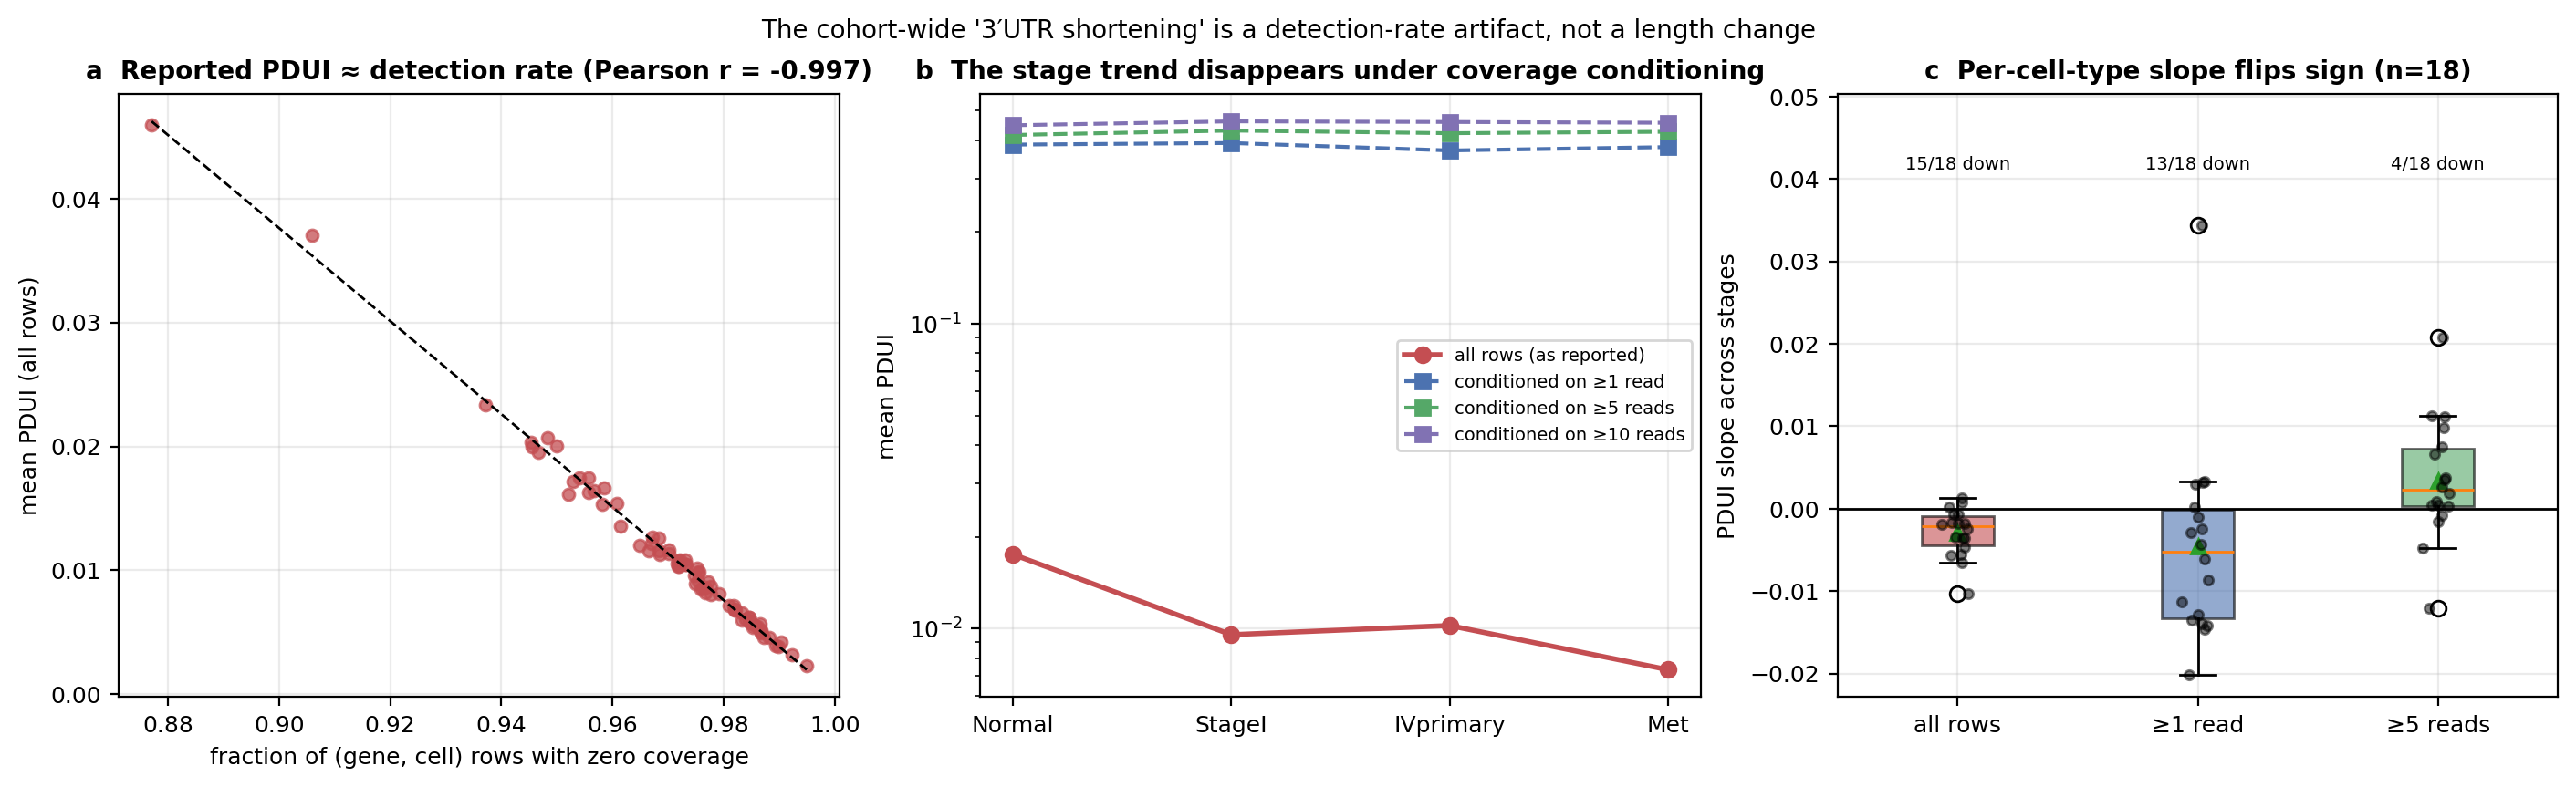
\includegraphics[width=\textwidth]{figures/corrected/06_depth_confound.png}
  \caption{(a) reported mean PDUI against the zero-coverage fraction, one point per
    (cell type, stage); (b) the stage trajectory unconditionally and under coverage
    conditioning; (c) per-cell-type stage slopes under each conditioning.}
  \label{fig:depth_confound}
\end{figure}

\begin{enumerate}
  \item \textbf{Reported PDUI is almost exactly the detection rate.} Across all 76
    (cell type, stage) observations, mean PDUI correlates with the zero-coverage
    fraction at Pearson $r = -0.997$ ($p = 3.9\times10^{-83}$; Spearman $-0.994$)
    and with mean reads per row at $r = +0.982$. Roughly 99\% of the variance in
    the quantity being interpreted as 3\textquotesingle{}UTR biology is explained
    by how often anything was detected at all.
  \item \textbf{Conditioning removes the trend.} Restricted to rows with $\geq$1
    read, mean PDUI is 0.387 / 0.392 / 0.370 / 0.380 across
    Normal $\rightarrow$ StageI $\rightarrow$ IVprimary $\rightarrow$ Met --- flat,
    and no longer correlated with depth ($r = -0.081$, $p = 0.48$). At $\geq$5 reads
    the ordering is 0.416 / 0.430 / 0.422 / 0.426: if anything the metastatic
    samples sit \emph{above} normal.
  \item \textbf{The sign of the per-cell-type slope is not robust.} Using all rows,
    15/18 cell types with $\geq$3 stages trend downward (Wilcoxon
    $p = 3.3\times10^{-4}$). At $\geq$1 read it is 13/18 ($p = 0.034$). At $\geq$5
    reads it is \textbf{4/18} --- the effect reverses, with mean slope $+0.0034$.
\end{enumerate}

\begin{quote}
\textbf{Conclusion.} The cohort-level direction of 3\textquotesingle{}UTR length
change is determined by the coverage threshold, not by the data. The reported
shortening is a restatement of the fact that metastatic and late-stage libraries in
this cohort are shallower per cell. \textbf{No claim of global
3\textquotesingle{}UTR shortening in this dataset is supportable}, and the magnitude
($|\text{slope}| \approx 0.003$ on a 0--1 scale) would be negligible even if the
direction held. What would rescue a length claim: per-gene tests restricted to genes
with adequate coverage in \emph{both} compared stages, with depth explicitly modelled
as a covariate, on cells matched for library size. That analysis is not in this sweep.
\end{quote}

\subsection{Stage Trajectory per Cell Type}

\begin{figure}[htbp]
  \centering
  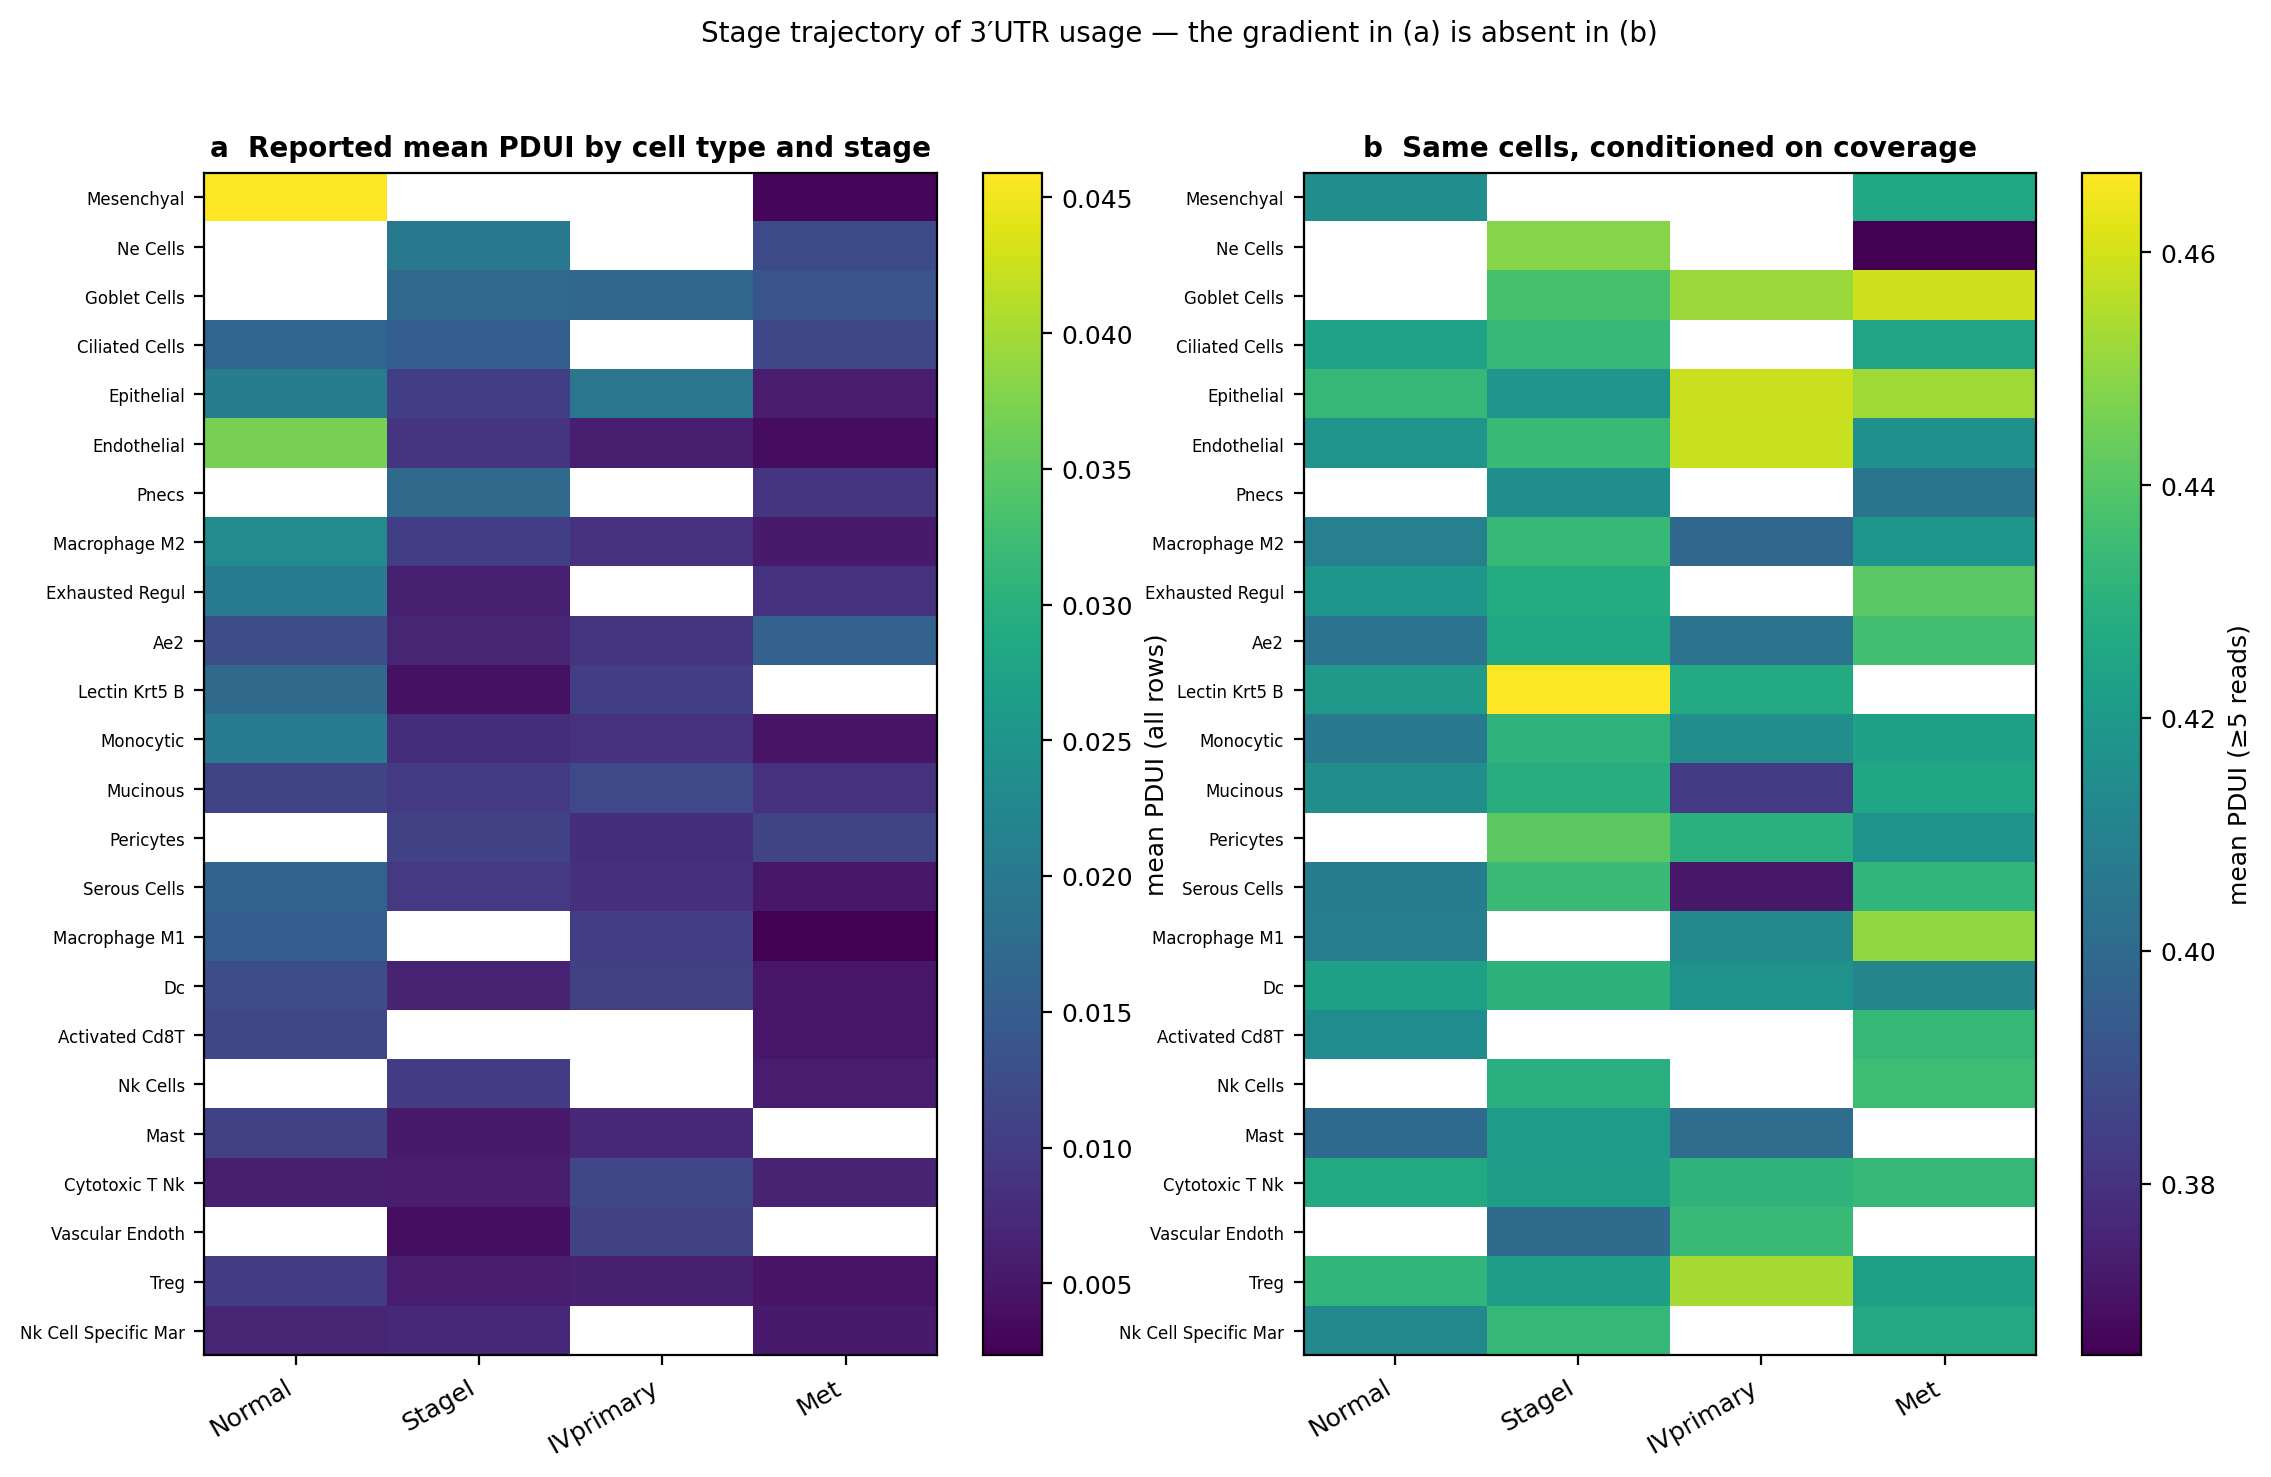
\includegraphics[width=\textwidth]{figures/corrected/07_stage_trajectory.png}
  \caption{Mean PDUI by cell type and stage, as reported (a) and conditioned on
    $\geq$5 reads (b), same cells and same ordering. The gradient in (a) is the
    detection-rate gradient; it is absent in (b).}
  \label{fig:stage_trajectory}
\end{figure}

The cell types with the steepest apparent shortening --- mesenchymal
($0.046 \rightarrow 0.003$), endothelial ($0.037 \rightarrow 0.004$), macrophage~M2
($0.023 \rightarrow 0.005$) --- are those with the largest drop in per-cell coverage
between Normal and Met. Cell types are also unevenly represented across stages: 8 of
24 lack at least one stage entirely, so several ``trends'' are two-point slopes.
Mesenchymal, the steepest of all, is fitted on \emph{two} stages.

\subsection{Differential-APA Significance Indexes Power, Not Effect}

\begin{figure}[htbp]
  \centering
  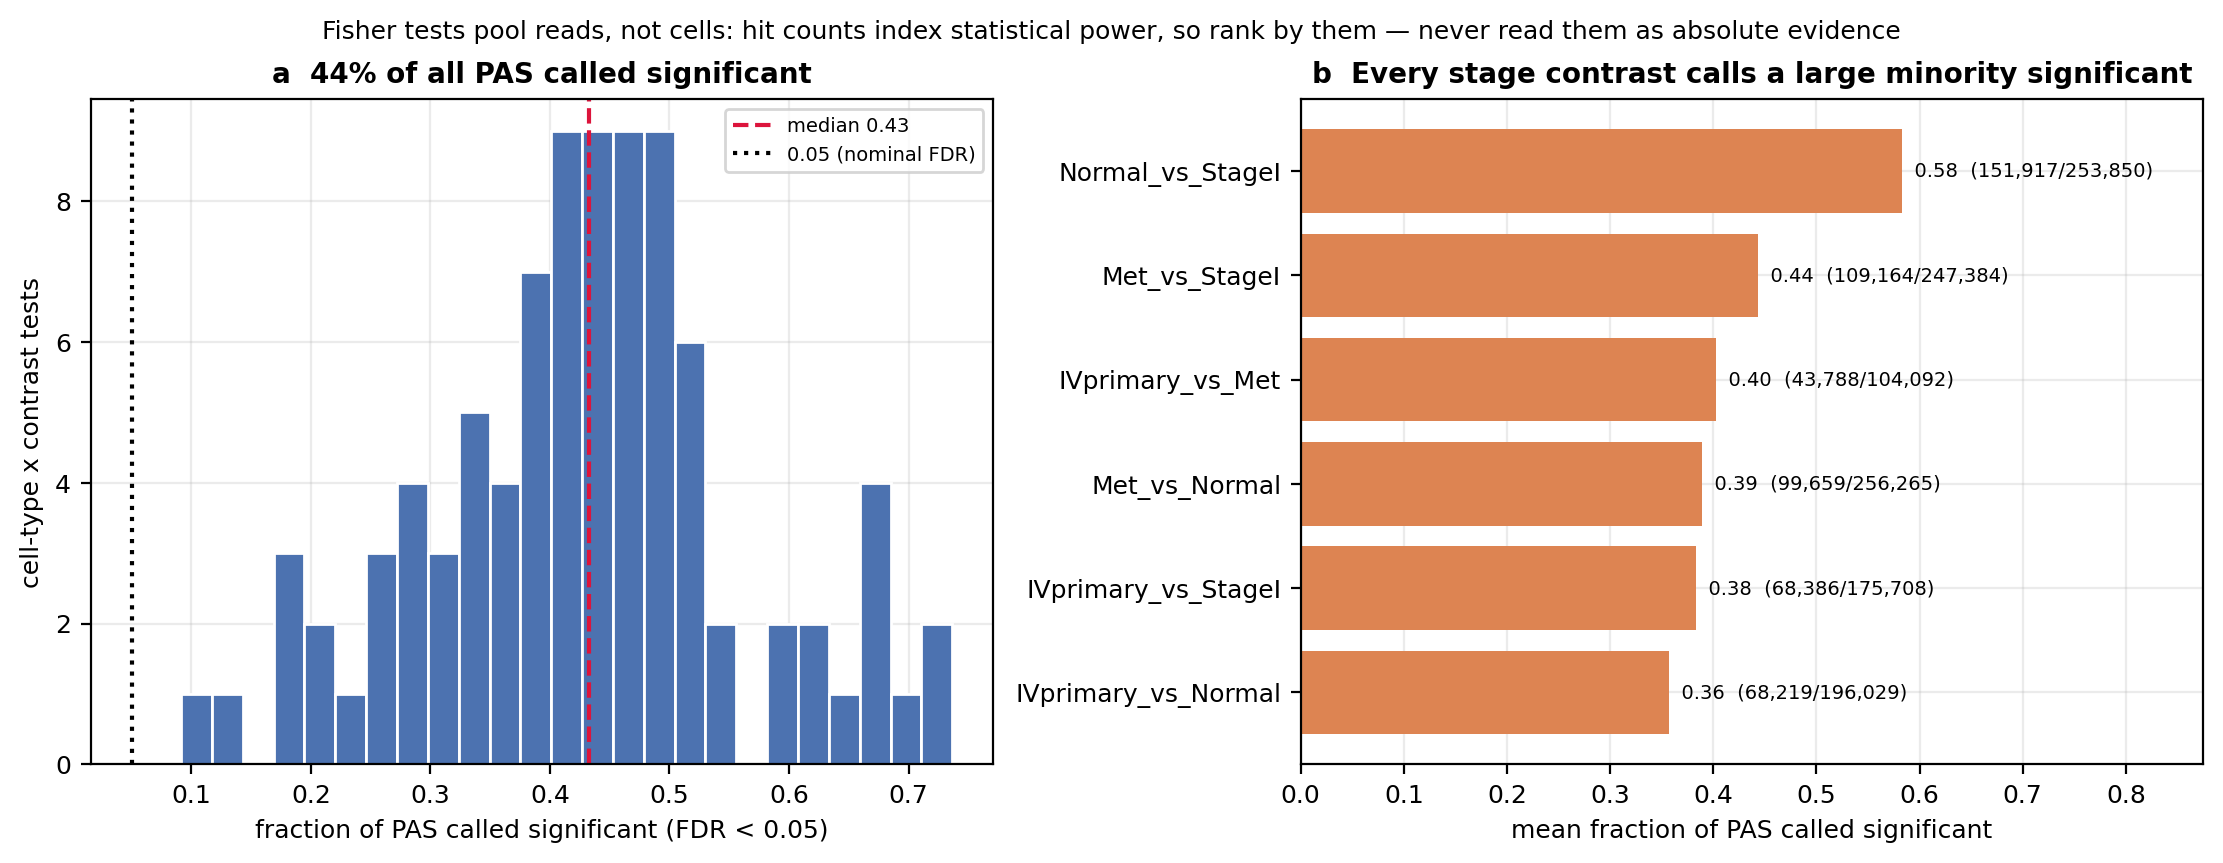
\includegraphics[width=\textwidth]{figures/corrected/08_fisher_power.png}
  \caption{(a) distribution of the per-(cell type, contrast) significance rate;
    (b) mean significance rate by stage contrast.}
  \label{fig:fisher_power}
\end{figure}

Across 1,233,328 Fisher tests, \textbf{541,133 (43.9\%) are significant at
FDR $< 0.05$}. A finding that 44\% of all polyadenylation sites are differentially
used between two stages of the same tumour is not biologically credible. It is the
expected signature of \textbf{pseudoreplication}: the Fisher contingency table is
built over \emph{reads}, so the effective sample size is read depth rather than the
number of cells or patients. Adding sequencing depth to the same biological material
increases significance without adding evidence; the project has separately measured
this dependence at $\rho = +0.68$.

\begin{table}[htbp]
  \centering
  \small
  \begin{tabular}{lrrrr}
    \toprule
    contrast & cell types & tests & significant & mean fraction \\
    \midrule
    Normal vs StageI    & 15 & 253,850 & 151,917 & 0.583 \\
    Met vs StageI       & 18 & 247,384 & 109,164 & 0.444 \\
    Met vs Normal       & 16 & 256,265 &  99,659 & 0.389 \\
    IVprimary vs Met    & 13 & 104,092 &  43,788 & 0.403 \\
    IVprimary vs StageI & 15 & 175,708 &  68,386 & 0.384 \\
    IVprimary vs Normal & 13 & 196,029 &  68,219 & 0.357 \\
    \bottomrule
  \end{tabular}
  \caption{Fisher significant-PAS hit counts by stage contrast.}
  \label{tab:fisher_hits}
\end{table}

Two consequences: \textbf{rank, never threshold} --- hit counts order cell types and
contrasts by how much evidence was available, and do not license ``gene~X is
differentially polyadenylated between Normal and Met''; and \textbf{the largest
contrast is the best-powered one, not the most different} --- Normal vs StageI tops
the table at 58.3\%, and Normal and Stage~I are also the two deepest strata.

\subsection{Recurrent versus Cell-Type-Private Switches}

\begin{figure}[htbp]
  \centering
  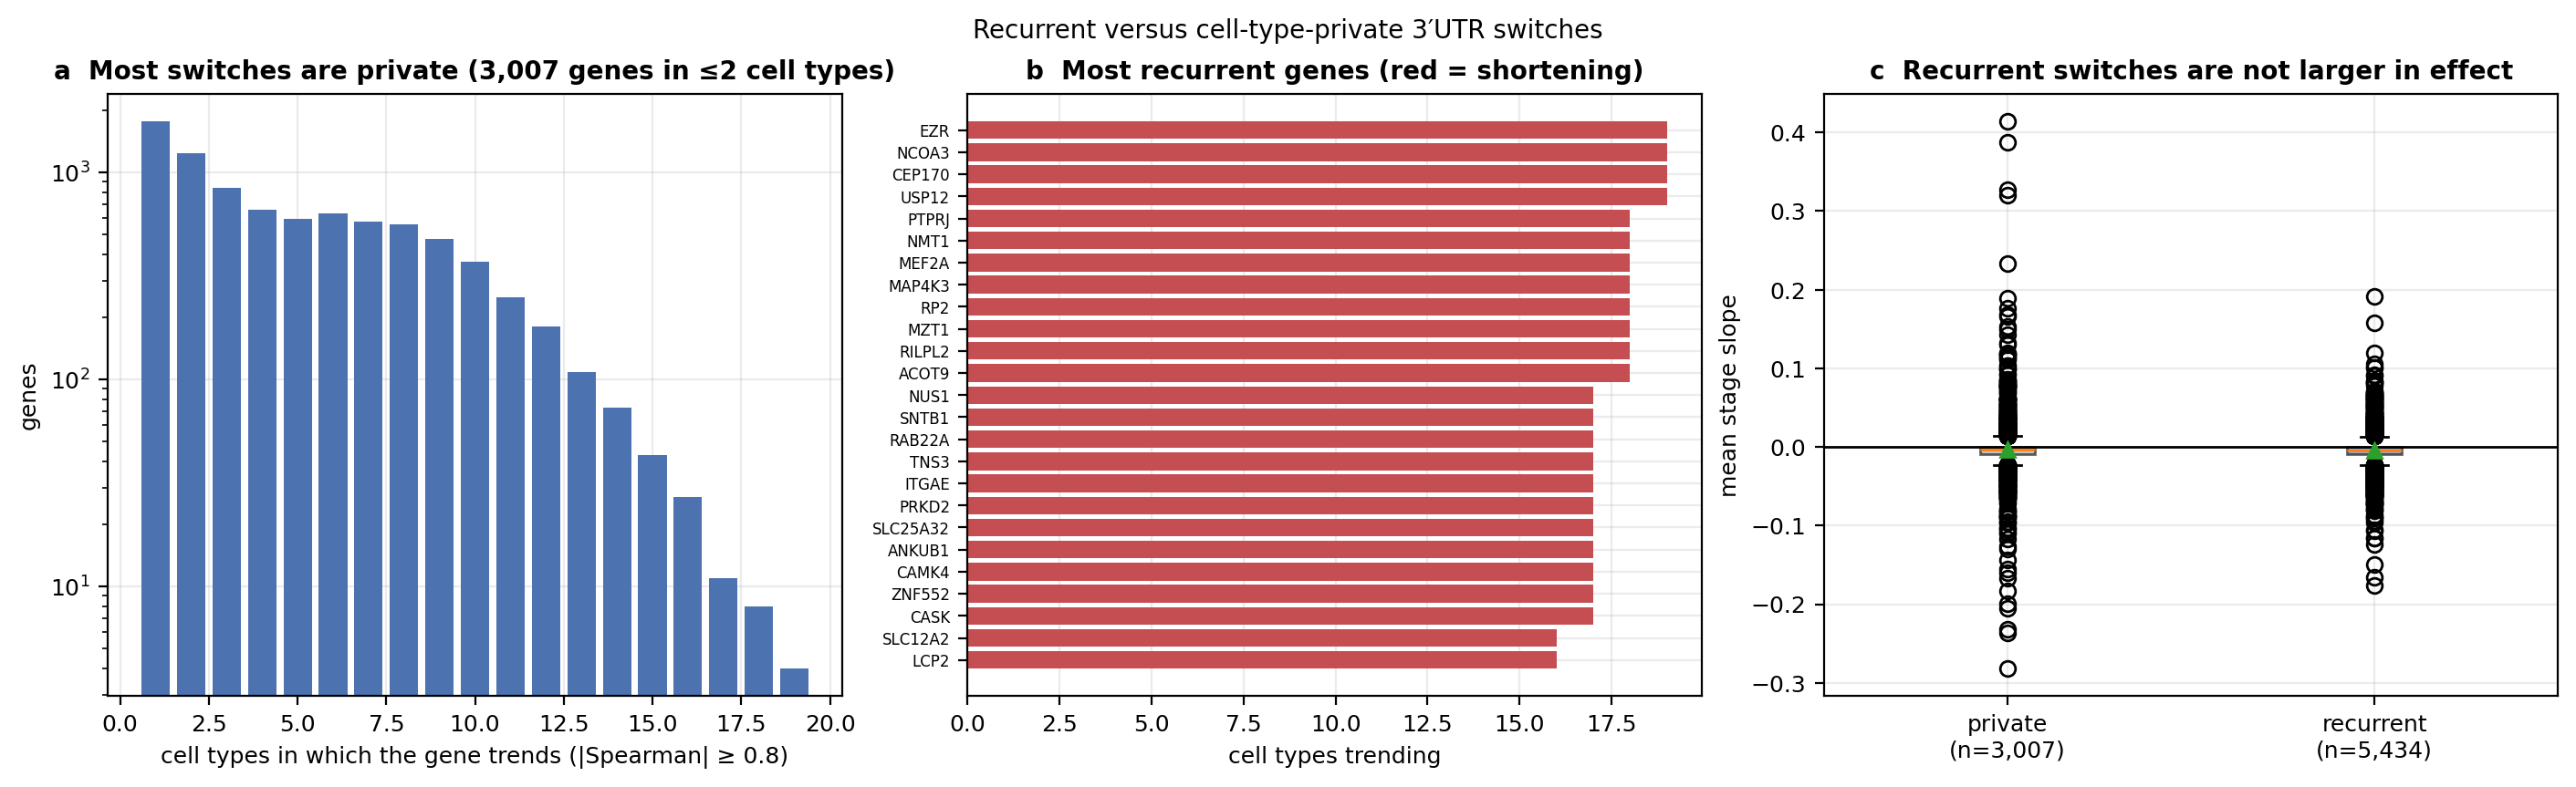
\includegraphics[width=\textwidth]{figures/corrected/09_recurrence.png}
  \caption{(a) how many cell types each gene trends in; (b) the 25 most recurrent
    genes; (c) effect size of recurrent versus private genes.}
  \label{fig:recurrence}
\end{figure}

Using the per-gene stage-trend tables across all 24 cell types (8,441 genes with at
least one trend call; $|\text{Spearman}| \geq 0.8$ defines ``trending''):

\begin{itemize}
  \item \textbf{3,007 genes (35.6\%) are private}, trending in $\leq$2 cell types.
  \item \textbf{5,434 genes trend in $\geq$3} cell types; of these 4,915 (90.5\%) are
    dominantly decreasing, with median direction consistency 0.857.
  \item The most recurrent genes (19 of $\leq$24 cell types) are \textbf{EZR, NCOA3,
    CEP170, USP12}, followed at 18 by \textbf{NMT1, MEF2A, MAP4K3, RP2, MZT1,
    RILPL2, ACOT9, PTPRJ}. Symbols are resolved from the exact GTF the run used
    (Ensembl GRCh38.99), not inferred.
  \item \textbf{Recurrence is not driven by effect size.} Private genes have
    \emph{larger} mean $|$slope$|$ than recurrent ones (0.0137 vs 0.0104;
    Mann--Whitney $p = 0.029$) --- the opposite of what a real shared biological
    program would produce, and what is expected if private calls are noisier
    estimates from fewer cells.
\end{itemize}

The honest reading is that recurrence here measures \textbf{testability}, not shared
regulation: a gene trends in many cell types largely when it is detected in many cell
types. The number of cell types in which a gene is even tested ranges from 1 to 24
(median 10), so \texttt{n\_celltypes\_trending} must be read against
\texttt{n\_celltypes\_tested}. Individual genes also carry internally inconsistent
summaries (PTPRJ is dominantly decreasing in 15/18 cell types yet has mean slope
$+0.030$), because a small number of saturated $0\rightarrow1$ flips dominate the
mean. Given Section~\ref{sec:corrected}, none of these genes should be described as
``shortening in LUAD progression''; they are the genes whose PAS usage is measurable
across the most cell types --- a candidate list for a properly depth-controlled
re-analysis, not a result.

\subsection{Does the Lost Distal 3\textquotesingle{}UTR Carry Regulatory Elements?}

The mechanistic story attached to 3\textquotesingle{}UTR shortening (Mayr \& Bartel
2009; Sandberg 2008) is that the removed distal segment carries miRNA sites and
AU-rich elements, so losing it de-represses the transcript. That is a sequence
claim, testable directly against the genome the run used.

For every gene with a proximal/distal PAS pair in the classic PDUI layer
($n = 3{,}641$), the segment between the two sites --- present only in the long
isoform --- was extracted from the GRCh38 primary assembly in mRNA-sense
orientation, together with a \textbf{length-matched control} immediately upstream
of the proximal PAS. Both were scanned for the class-II ARE pentamer
\texttt{ATTTA}, the \texttt{WTTTATTTAW} nonamer, and 7mer-m8 seed matches for six
miRNA families (seeds computed in code from the mature sequences).

\begin{figure}[htbp]
  \centering
  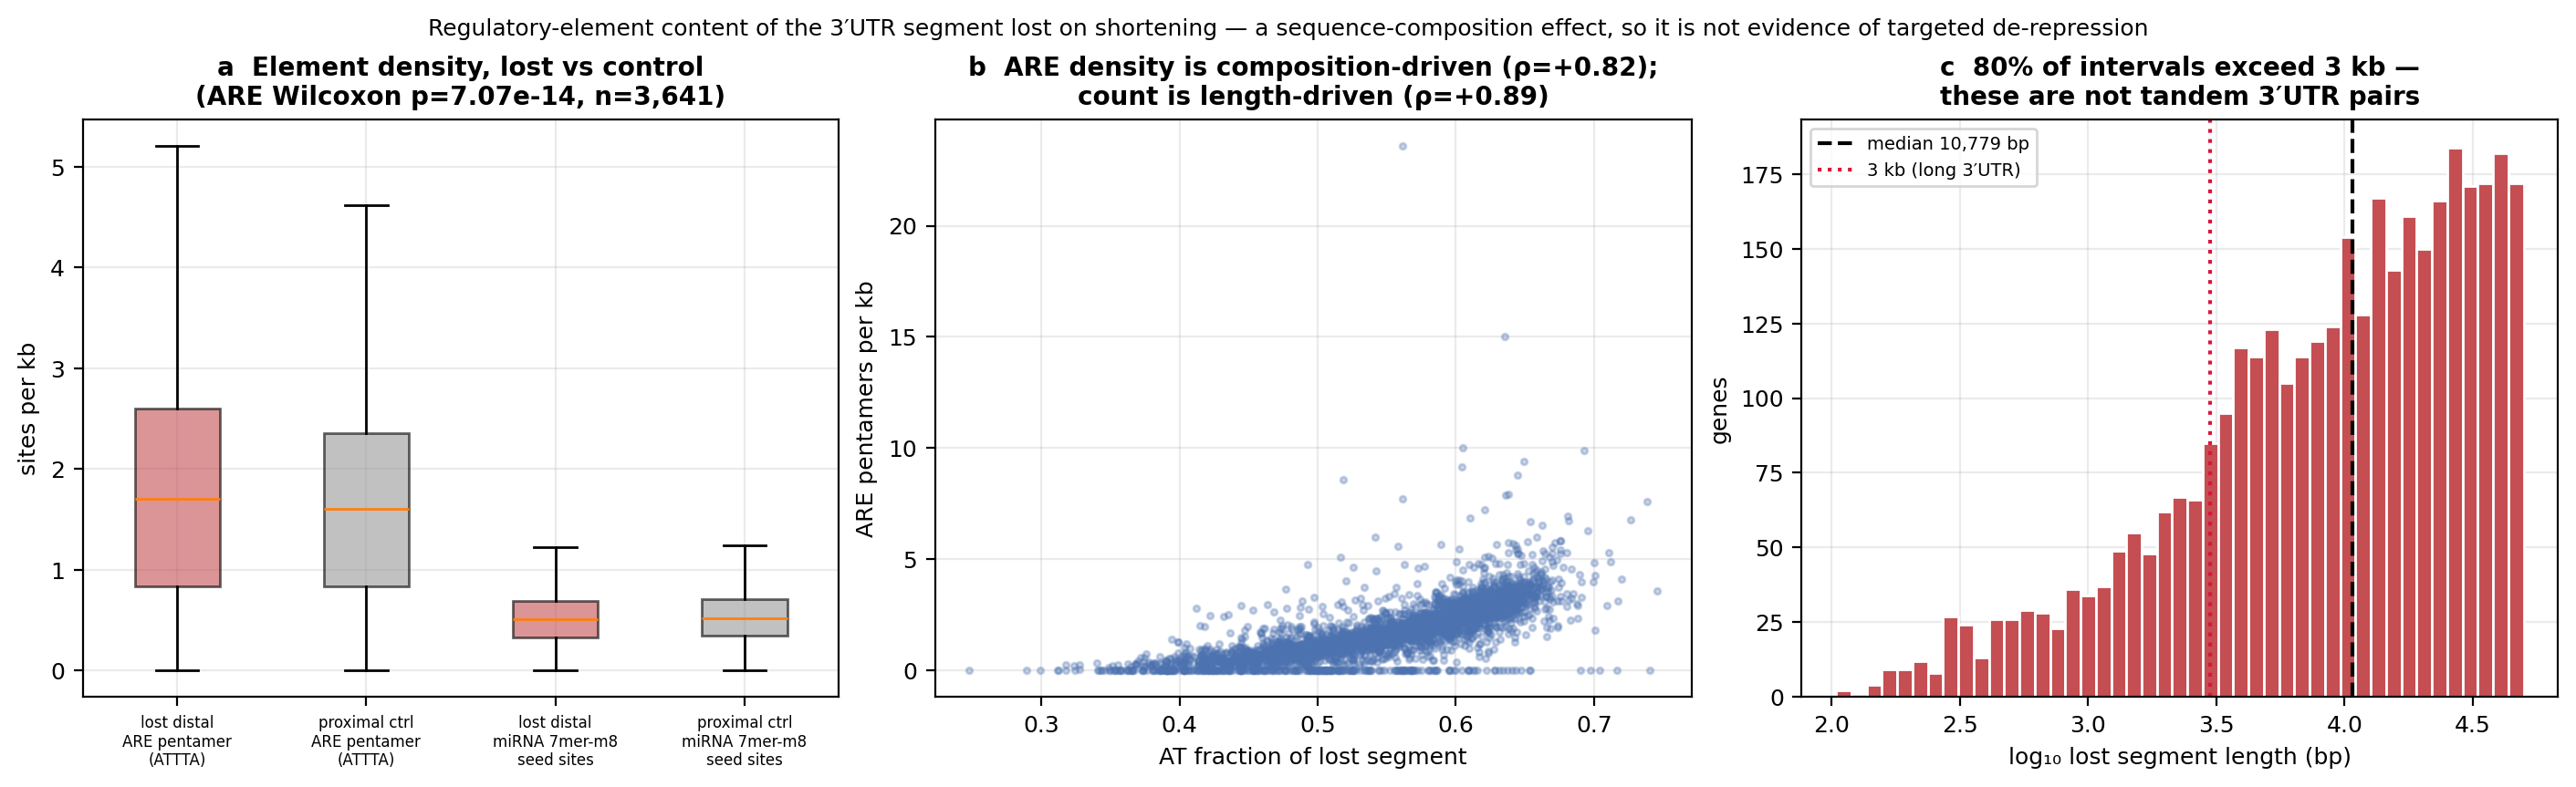
\includegraphics[width=\textwidth]{figures/corrected/10_lost_distal_elements.png}
  \caption{(a) element density in the lost segment versus the length-matched
    proximal control; (b) ARE density against AT content; (c) length distribution
    of the intervals being scanned.}
  \label{fig:lost_distal}
\end{figure}

\begin{table}[htbp]
  \centering
  \small
  \begin{tabular}{lrrr}
    \toprule
    measure & lost (median) & control (median) & Wilcoxon $p$ \\
    \midrule
    ARE pentamer, count       & 16.0  & 17.0  & $4.8\times10^{-18}$ \\
    ARE pentamer, per kb      & 1.703 & 1.603 & $7.1\times10^{-14}$ \\
    ARE nonamer, count        & 1.0   & 0.0   & 0.63 \\
    miRNA 7mer-m8, count      & 6.0   & 6.0   & $4.1\times10^{-3}$ \\
    miRNA 7mer-m8, per kb     & 0.510 & 0.520 & \textbf{0.058} \\
    AT fraction               & 0.562 & 0.548 & $1.4\times10^{-53}$ \\
    \bottomrule
  \end{tabular}
  \caption{Regulatory-element content of the lost distal segment versus a
    length-matched proximal control.}
  \label{tab:lost_distal}
\end{table}

\textbf{The mechanism is not supported by this data.}

\begin{enumerate}
  \item \textbf{No miRNA-site enrichment.} Seed-site density in the lost segment is
    0.510/kb versus 0.520/kb in the control --- statistically indistinguishable
    ($p = 0.058$) and pointing the \emph{wrong way}.
  \item \textbf{The ARE excess is a composition effect.} ARE density is nominally
    higher in the lost segment (1.70 vs 1.60 per kb) and the $p$-value is small
    because $n$ is large, but the effect is 6\% relative. It is fully accounted for
    by the lost segment being slightly more AT-rich (0.562 vs 0.548): ARE density
    tracks AT fraction at Spearman $\rho = +0.82$, and raw ARE count tracks segment
    length at $\rho = +0.89$. The functional nonamer shows no difference at all
    ($p = 0.63$).
  \item \textbf{The interval being scanned is mostly not 3\textquotesingle{}UTR.}
    The median proximal-to-distal span is \textbf{10,779\,bp} (IQR 3,867--24,497),
    and \textbf{80\% exceed 3\,kb} --- longer than almost any real human
    3\textquotesingle{}UTR. These PAS pairs are therefore not predominantly tandem
    3\textquotesingle{}UTR sites; many span introns or whole gene bodies.
\end{enumerate}

Point 3 is a \textbf{pipeline finding, not a biology finding}: the classic PDUI
layer is pairing PAS that are too far apart to be a tandem UTR pair. Restricting
PDUI to proximal/distal pairs within the annotated 3\textquotesingle{}UTR of the
same transcript --- which the GTF already provides --- is a prerequisite for any
length or mechanism claim. Until that is done the de-repression mechanism can be
neither supported nor refuted here; what can be said is that the current intervals
show no targeted regulatory-element loss beyond sequence composition.

\begin{quote}
\textbf{Scope of this test.} A seed-match scan is an upper bound on candidate
sites: it ignores site conservation, 3\textquotesingle{}UTR accessibility, and the
context features TargetScan models, and it does not weight by miRNA expression. It
is used here in the direction it is valid --- a \emph{negative} result (no
enrichment) is meaningful, whereas a positive one would have needed follow-up.
\end{quote}

\subsection{Cancer-Gene and Pathway Themes of the Recurrent Switch Genes}

The biological-findings report leans on two claims never tested against a
background: that the switch genes are enriched for known cancer genes, and that
they share pathway themes. Both are testable, and both are \textbf{negative} once
the confound from Section~\ref{fig:recurrence} is handled.

Reference sets are fetched from public endpoints and cached: the \textbf{OncoKB
cancer gene list} (1,245 genes, carrying the \texttt{sangerCGC} flag --- membership
of the \textbf{COSMIC Cancer Gene Census}, 581 genes --- plus ONCOGENE/TSG typing)
and the \textbf{50 MSigDB Hallmark} sets.

\textbf{The confound.} Recurrence tracks \emph{detectability}, detectability is
driven by expression, and cancer-gene catalogues are themselves biased toward
well-studied, highly expressed genes. A ``recurrent genes vs all genes'' test would
recover expression bias and report it as cancer biology. Two guards: the universe
is restricted to the 8,441 genes carrying a trend call, and detectability
(\texttt{n\_celltypes\_tested}) is adjusted for by logistic regression.

\begin{figure}[htbp]
  \centering
  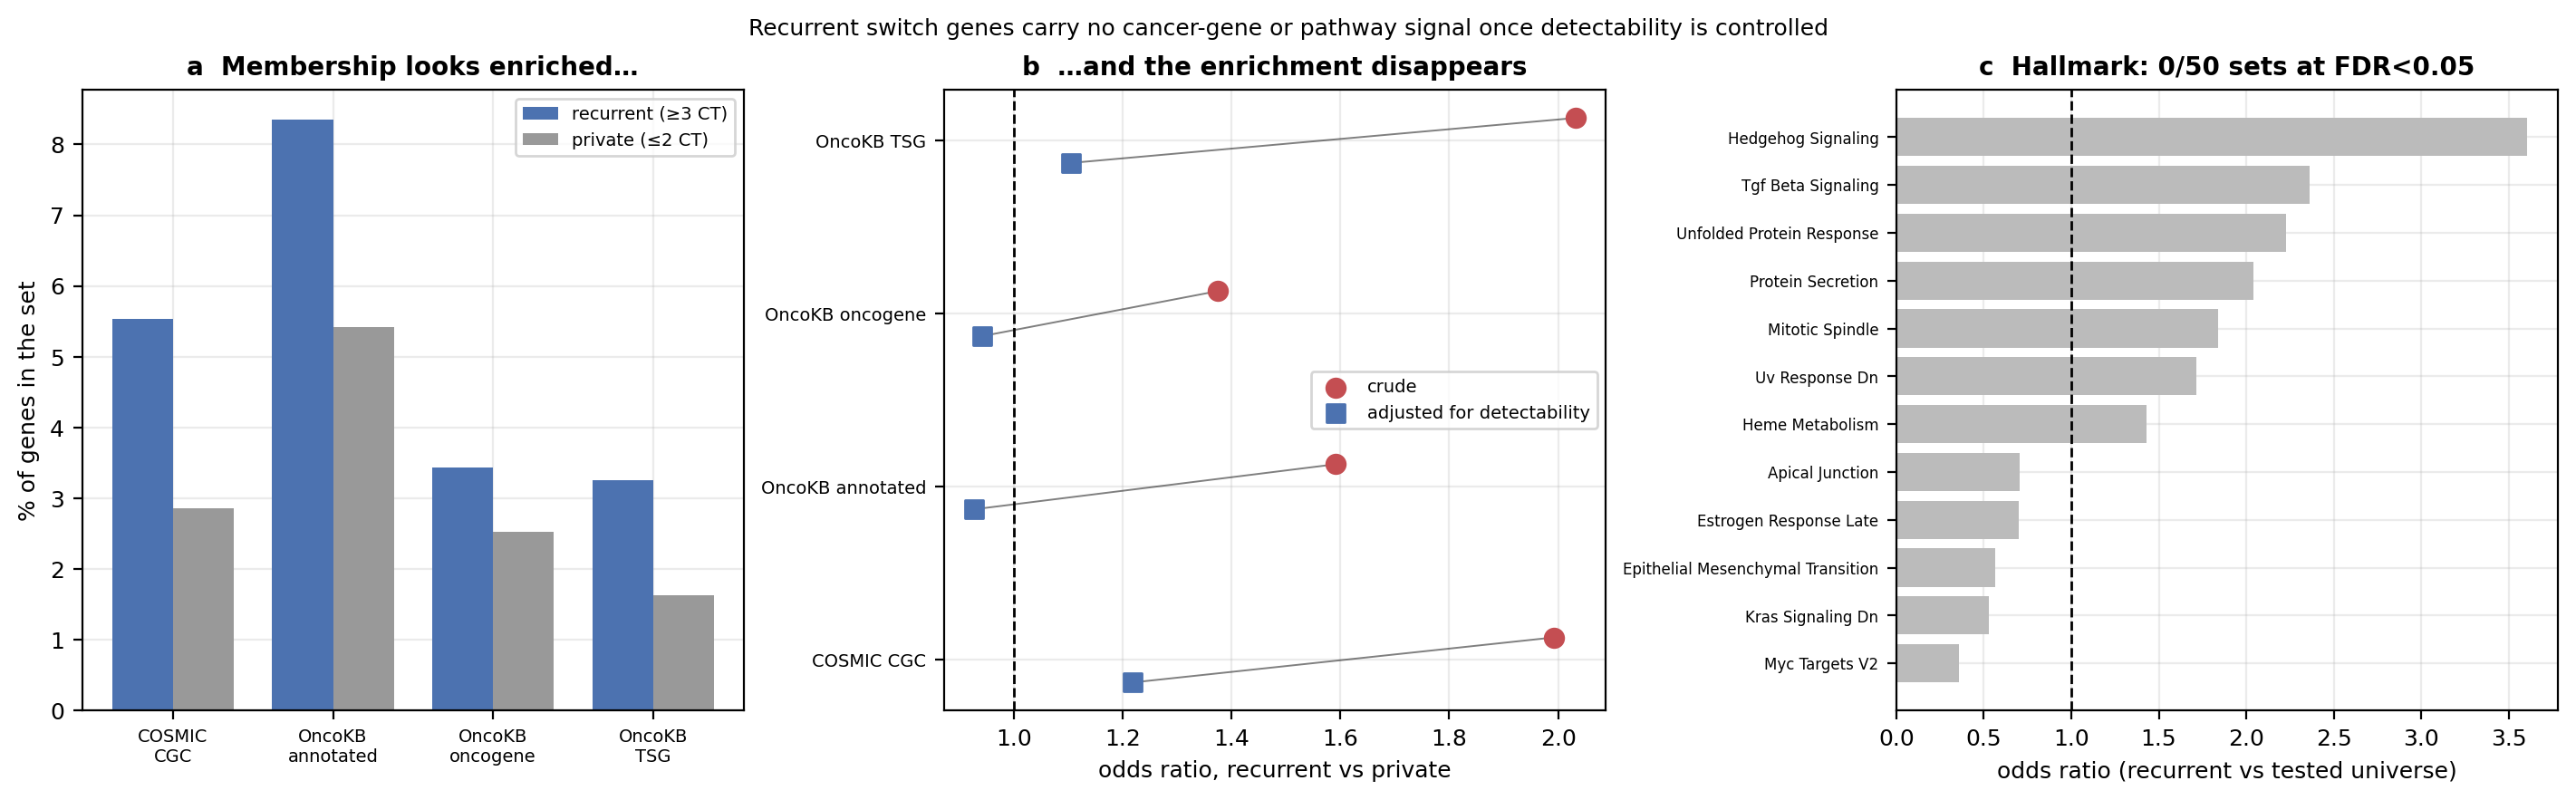
\includegraphics[width=\textwidth]{figures/corrected/11_gene_sets.png}
  \caption{(a) raw membership rates; (b) crude versus detectability-adjusted odds
    ratios; (c) Hallmark enrichment of the recurrent set against the tested
    universe.}
  \label{fig:gene_sets}
\end{figure}

\begin{table}[htbp]
  \centering
  \small
  \begin{tabular}{lrrrrrr}
    \toprule
    gene set & recurrent & private & crude OR & $p$ & adj.\ OR & $p$ \\
    \midrule
    COSMIC CGC       & 5.54\% & 2.86\% & 1.99 & $6.7\times10^{-9}$ & \textbf{1.22} & \textbf{0.28} \\
    OncoKB annotated & 8.36\% & 5.42\% & 1.59 & $4.8\times10^{-7}$ & \textbf{0.93} & \textbf{0.60} \\
    OncoKB oncogene  & 3.44\% & 2.53\% & 1.37 & 0.022             & \textbf{0.94} & \textbf{0.78} \\
    OncoKB TSG       & 3.26\% & 1.63\% & 2.03 & $5.7\times10^{-6}$ & \textbf{1.10} & \textbf{0.68} \\
    \bottomrule
  \end{tabular}
  \caption{Cancer-gene membership of recurrent versus private switch genes, crude
    and adjusted for detectability.}
  \label{tab:cancer_genes}
\end{table}

\textbf{Every apparent enrichment is accounted for by how many cell types could
test the gene.} The crude odds ratios look convincing --- a doubling of Cancer Gene
Census membership at $p = 6.7\times10^{-9}$ is exactly the kind of number that gets
reported as a finding. After adjusting for detectability all four collapse to the
null, two below 1.0.

\textbf{No pathway themes either.} Of the 50 Hallmark sets, \textbf{0 reach
FDR $< 0.05$}. The nominally strongest are Mitotic Spindle (OR 1.84, $q = 0.080$),
Unfolded Protein Response (OR 2.23, $q = 0.097$) and Protein Secretion (OR 2.04,
$q = 0.097$) --- none survives multiple testing, and all three are high-expression
housekeeping-adjacent programs, which is what detectability bias predicts.

\textbf{Direction carries no oncogene/TSG asymmetry.} If shortening de-repressed
oncogenes, shortening genes should skew oncogene and lengthening genes skew tumour
suppressor. They do not: shortening splits 236 oncogenes to 205 TSGs, lengthening
27 to 21 (OR 0.90, $p = 0.76$) --- expected, since direction is a detection-rate
artifact and cannot carry a functional signal.

\begin{quote}
\textbf{Why the matched-resampling control is reported but not used.} A
detectability-matched null is also computed, and flagged \textbf{UNRELIABLE}:
recurrent and private genes barely overlap on \texttt{n\_celltypes\_tested}
(median \textbf{18 vs 2}; strata 17--24 hold 3,337 recurrent genes against
\textbf{30} private ones). Resampling from strata of 2--3 genes gives a ``null''
fixed by a handful of genes, which is why that column disagrees with itself across
sets. The near-total non-overlap is the point: recurrence and detectability are
close to the same variable here. The logistic adjustment is the primary result
because it is stable, but it adjusts across a thin overlap region, so its null
should be read as ``no evidence of enrichment,'' not a precise zero.
\end{quote}

\textbf{Consequence for the biological narrative.} The curated
oncogene-shortening / tumour-suppressor-lengthening tables in
\texttt{PeakATail\_Laughney\_Biological\_Findings.md} have no statistical support
at the cohort level. Individual genes there may still be real, but they were
selected by inspection from a set with no detectable enrichment, so the selection
cannot be justified by the aggregate.

% -----------------------------------------------------------------------------
\section{Experiment Matrix --- What Was Run, and With Which Parameters}
\label{sec:matrix}
% -----------------------------------------------------------------------------

Every row is reconstructed from the runs themselves
(\texttt{reports/build\_experiment\_matrix.py} reads the 19
\texttt{run\_manifest.json} files and their \texttt{resolved\_config}), not from
the sweep definition, so it records what the pipeline \emph{did} rather than what
it was asked to do. Full per-run parameters (46 fields) are in
\texttt{cumulative\_analysis/experiment\_matrix.csv}.

\textbf{Common to all runs:} GTF \texttt{Homo\_sapiens.GRCh38.99.gtf}; atlas
\texttt{polyasite\_3.0\_GRCh38\_ensembl\_sorted.bed} at
\texttt{atlas\_distance = 50}; \texttt{merge\_strategy: before} per dataset; the
\texttt{original} peak strategy excluded throughout.

\begin{table}[htbp]
  \centering \small
  \begin{tabular}{llllrrlrrr}
    \toprule
    run & strategy & atlas & ip mode & maxPAS & $\lambda$ win & $\lambda$ method & FC & gap & prom \\
    \midrule
    \texttt{lg\_ip\_filter} & lambda\_gradient & annotate & filter & 5 & 5000 & median & 2.0 & 100 & 5.0 \\
    \texttt{lg\_ip\_off} & lambda\_gradient & annotate & off & 5 & 5000 & median & 2.0 & 100 & 5.0 \\
    \texttt{lp\_annotate} & lambda\_poisson & annotate & annotate & 5 & 5000 & median & 2.0 & 100 & 5.0 \\
    \texttt{si\_annotate} & sierra\_iterative & annotate & annotate & 5 & 5000 & median & 2.0 & 100 & 5.0 \\
    \texttt{lg\_annotate} & lambda\_gradient & annotate & annotate & 5 & 5000 & median & 2.0 & 100 & 5.0 \\
    \bottomrule
  \end{tabular}
  \caption{A. Peak-calling grid (5 runs, full 17-dataset cohort input).}
  \label{tab:matrix_peak}
\end{table}

\begin{table}[htbp]
  \centering \small
  \begin{tabular}{lrrl}
    \toprule
    branch & max\_gene\_distance & utr\_multiplier & include\_extended \\
    \midrule
    \texttt{A2\_trim\_d10000\_ext} & 10000 & 2.0 & yes \\
    \texttt{A2\_trim\_d1000\_ext} & 1000 & 2.0 & yes \\
    \texttt{A2\_trim\_d2000\_ext} & 2000 & 2.0 & yes \\
    \texttt{A2\_trim\_d3000\_ext} & 3000 & 2.0 & yes \\
    \texttt{A2\_trim\_d5000\_ext} & 5000 & 2.0 & yes \\
    \texttt{A2\_trim\_default} & 5000 & 2.0 & no \\
    \texttt{A2\_trim\_mult1.5} & 5000 & 1.5 & no \\
    \texttt{A2\_trim\_mult3.0} & 5000 & 3.0 & no \\
    \bottomrule
  \end{tabular}
  \caption{B. Trim / annotation-window branches.}
  \label{tab:matrix_trim}
\end{table}

\begin{table}[htbp]
  \centering \small
  \begin{tabular}{llrr}
    \toprule
    branch & method & resolution & n\_neighbors \\
    \midrule
    \texttt{A3\_libsize} & leiden\_libsize & 1.0 & 30 \\
    \texttt{A3\_nn15} & leiden\_tfidf & 1.0 & 15 \\
    \texttt{A3\_nn50} & leiden\_tfidf & 1.0 & 50 \\
    \texttt{A3\_res0.5} & leiden\_tfidf & 0.5 & 30 \\
    \texttt{A3\_res2.0} & leiden\_tfidf & 2.0 & 30 \\
    \bottomrule
  \end{tabular}
  \caption{C. Clustering branches.}
  \label{tab:matrix_clust}
\end{table}

\noindent\textbf{D. Cell-level filters}, identical across all runs:
\texttt{min\_read = 1500}, \texttt{min\_cells = 3}, \texttt{min\_genes = 50},
\texttt{min\_pas\_per\_cell = 50}.

\medskip
\noindent\textbf{E. Cohort and switch layer.} 17 GSM libraries
(\texttt{B1\_cohort\_full}), 8 BAMs each, spanning Normal / StageI (IA, IB, IIA) /
IVprimary / Met (bone, brain); 24 signature-scored cell types; GEX cross-check in
\texttt{B2\_gex\_celltyping}; switch layers \texttt{B3\_switch/\{diff, length,
trend\}}. Diff strategies: \texttt{fisher} (6 stage contrasts) and
\texttt{nb\_multi} (omnibus). Length strategies: \texttt{classic},
\texttt{proportion}, \texttt{shannon}. Note that \textbf{\texttt{nb\_pairwise} was
not run}, so the three-way diff-strategy comparison in the superseded Figure~17
cannot be reproduced.

\subsection{Two Provenance Traps Worth Recording}

\begin{enumerate}
  \item \textbf{\texttt{ip\_filter\_mode} does not identify the internal-priming
    arm.} It remains \texttt{"annotate"} even when the filter is disabled; the
    real switch is the boolean \texttt{ip\_filter}. This also explains the
    Jaccard $= 1.000$ between \texttt{lg\_annotate} and \texttt{lg\_ip\_off}: in
    \texttt{annotate} mode the filter only \emph{labels} peaks and removes none,
    so disabling it produces byte-identical output. The nominally three-level ip
    axis is really two-level.
  \item \textbf{The re-annotation branches' manifests describe their base run.}
    \texttt{A2\_*} and \texttt{A3\_*} re-annotate an existing run, so their
    manifests carry the \emph{base} run's args. Read naively, all eight trim
    branches report \texttt{max\_gene\_distance = 5000} and every clustering
    branch \texttt{resolution = 1.0} --- the varied axis disappears. For those 13
    runs \texttt{trim\_cluster\_grid.tsv} is authoritative. Any future audit
    reading only the manifests will silently conclude these branches were
    identical.
\end{enumerate}

\subsection{Defined but Not Executed}

The \texttt{sweep\_grid.tsv} filter-threshold arm (18 \texttt{SWb\_*} branches)
was defined but \textbf{never run}. The cell-level filters are therefore fixed at
a single setting throughout, and no claim in this report rests on a
filter-threshold sensitivity analysis. Sensitivity to \texttt{max\_gene\_distance}
and \texttt{utr\_multiplier} \emph{is} covered by the \texttt{A2\_*} branches.

% -----------------------------------------------------------------------------
\section{Filter-Effect Comparison --- Pending}
\label{sec:filter_effect}
% -----------------------------------------------------------------------------

\begin{quote}
\textbf{Status: experiment running; this section is a placeholder and contains no
results.} Nothing here may be cited until it is filled in.
\end{quote}

A separate run is executing the \textbf{full pipeline} (peak calling
$\rightarrow$ clustering $\rightarrow$ GEX cell-typing $\rightarrow$ switch
\texttt{diff} + \texttt{length} + \texttt{trend}) on the 6-GSM subset under four
filtering scenarios --- baseline (label only), atlas-filter, annot-filter (GTF
3\textquotesingle{}UTR), and ip-filter --- to measure how each filter propagates
to the biological readout rather than only to peak counts. It will report, per
scenario: PAS retained and cluster structure (n clusters, ARI/AMI against GEX
labels); differential-APA hit counts by stage contrast; and the
shortening/lengthening split with its slope distribution.

\textbf{Why this matters.} Section~\ref{sec:validation} showed that F1 against a
saturated reference \emph{penalises} a filter that removes false positives, so
filters cannot be evaluated on atlas agreement. Whether a filter changes the
biology is the question that remains --- and Section~\ref{fig:lost_distal} gives a
concrete reason to expect the annot-filter to matter most: 80\% of the
proximal/distal PAS pairs driving PDUI span more than 3\,kb, which restricting to
the annotated 3\textquotesingle{}UTR would directly address.

Three predictions are recorded \textbf{in advance} so the result reads as a test:
clustering should be robust (trim grid moved it by only 0.24); differential hit
counts should fall roughly in proportion to PAS removed, if they index power
rather than effect; and the shortening/lengthening split should move most under
annot-filter, toward the depth-conditioned result of no consistent direction. If
the split is instead unchanged across all four scenarios, that strengthens the
conclusion that direction is set by coverage, not by which PAS are included.

\section{Figure Index}
\label{sec:figure_index}
% ─────────────────────────────────────────────────────────────────────────────

\begin{longtable}{rll}
  \toprule
  \textbf{\#} & \textbf{Description} & \textbf{File} \\
  \midrule
  \endhead
  1  & Strategy explained                    & \texttt{fig\_strategy\_explained.png} \\
  2  & Math methods                          & \texttt{fig\_math\_methods.png} \\
  3  & Peak counts                           & \texttt{fig\_peak\_counts.png} \\
  4  & Annotation impact                     & \texttt{fig\_annotation\_impact.png} \\
  5  & Dual DB validation                    & \texttt{fig\_dual\_db\_validation.png} \\
  6  & Precision metrics table               & \texttt{fig\_dual\_db\_table.png} \\
  7  & Precision by distance                 & \texttt{fig\_precision\_v3.png} \\
  8  & Distance histogram                    & \texttt{fig\_distance\_hist.png} \\
  9  & Strategy overlap Venn                 & \texttt{fig\_venn\_overlap.png} \\
  10 & Parameter sensitivity                 & \texttt{fig\_metrics\_table.png} \\
  11 & ARI/AMI resolution sweep              & \texttt{fig\_ari\_ami\_sweep.png} \\
  12 & 6-panel clustering comparison         & \texttt{fig\_main\_comparison.png} \\
  13 & Sankey flow diagram                   & \texttt{fig\_sankey.png} \\
  14 & Cluster sizes                         & \texttt{fig\_cluster\_sizes.png} \\
  15 & APA subclusters                       & \texttt{fig\_subcluster.png} \\
  16 & Differential APA (PDUI + volcano)     & \texttt{fig\_differential\_apa.png} \\
  17 & Switch strategy explainer (cartoon)   & \texttt{switch\_strategy\_explainer.png} \\
  18 & Length strategy explainer (cartoon)   & \texttt{length\_strategy\_explainer.png} \\
  23 & Match strategy explainer (cartoon)    & \texttt{match\_strategy\_explainer.png} \\
  19 & Switch strategy real-data comparison  & \texttt{switch\_strategy\_real\_data.png} \\
  20 & Length strategy real-data comparison  & \texttt{length\_strategy\_real\_data.png} \\
  21 & Gene walk: DPYD                       & \texttt{gene\_walk\_ENSG00000188641.png} \\
  22 & Gene walk: PHACTR1                    & \texttt{gene\_walk\_ENSG00000112137.png} \\
  \bottomrule
\end{longtable}

\end{document}
